\documentclass[11pt]{article}

% Switch to "final" or "preprint" before camera-ready / when posting to arXiv.
% [review] is anonymous; [preprint] keeps author names; [final] is
% the camera-ready version.
\usepackage[preprint]{acl}

% ── Standard ACL packages ─────────────────────────────────────
\usepackage{times}
\usepackage{latexsym}
\usepackage[T1]{fontenc}
\usepackage[utf8]{inputenc}
\usepackage{microtype}
\usepackage{inconsolata}
\usepackage{graphicx}

% ── Math + theorem environments ───────────────────────────────
\usepackage{amsmath}
\usepackage{amssymb}
\usepackage{amsfonts}
\usepackage{amsthm}
\usepackage{mathtools}

\theoremstyle{plain}
\newtheorem{theorem}{Theorem}[section]
\newtheorem{proposition}[theorem]{Proposition}
\theoremstyle{definition}
\newtheorem{definition}[theorem]{Definition}
\theoremstyle{remark}
\newtheorem{remark}[theorem]{Remark}

\DeclareMathOperator*{\argmin}{arg\,min}
\DeclareMathOperator*{\argmax}{arg\,max}

% ── Layout helpers ────────────────────────────────────────────
\usepackage{booktabs}
\usepackage{multirow}
\usepackage{enumitem}
\usepackage{xcolor}
\usepackage{algorithm}
\usepackage{algpseudocode}
\usepackage{tcolorbox}
\tcbuselibrary{skins, breakable}

% ── Verbatim listings (used for the LLM judge prompt appendix) ─
\usepackage{listings}
\lstdefinestyle{judgeprompt}{
  basicstyle=\footnotesize\ttfamily,
  frame=single,
  framerule=0.4pt,
  framesep=4pt,
  xleftmargin=4pt,
  xrightmargin=4pt,
  breaklines=true,
  breakatwhitespace=true,
  breakindent=0pt,
  showstringspaces=false,
  columns=fullflexible,
  upquote=true,
  literate={—}{{---}}1,
}

% ── Tikz for the conceptual figure (single full-width figure*) ─
\usepackage{tikz}
\usetikzlibrary{positioning, shapes.geometric, arrows.meta}

% ── Colours ───────────────────────────────────────────────────
\definecolor{myred}{RGB}{180,0,0}
\definecolor{myblue}{RGB}{0,70,160}
\definecolor{mygreen}{RGB}{0,120,50}
\definecolor{lightblue}{RGB}{230,240,255}
\definecolor{lightred}{RGB}{255,235,235}
\definecolor{lightgreen}{RGB}{235,255,240}

% ── Custom commands ───────────────────────────────────────────
\newcommand{\red}[1]{\textcolor{myred}{\textbf{#1}}}
\newcommand{\UniEdu}{\textsc{UnifiedEdu}}
\newcommand{\indiv}{\text{indiv}}
\newcommand{\fed}{\text{fed}}
\newcommand{\uni}{\text{uni}}

\newtcolorbox{scenariobox}{
  enhanced, breakable,
  colback=lightblue, colframe=myblue,
  fonttitle=\bfseries,
  title=Motivating Scenario, arc=4pt
}
\newtcolorbox{hypothesisbox}{
  enhanced, breakable,
  colback=lightblue, colframe=myblue,
  fonttitle=\bfseries\color{white},
  coltitle=white, colbacktitle=myblue,
  title=Main Hypothesis, arc=4pt
}

% ── Title ─────────────────────────────────────────────────────
\title{\UniEdu{}: Equitable Automated Q\&A Generation\\
       via Unified Federated Learning}

\author{
  Furkan Pala \and
  \red{[co-authors TBC]} \and
  Islem Rekik \\
  BASIRA Lab, Imperial-X (I-X) and Department of Computing \\
  Imperial College London, London, United Kingdom \\
  \texttt{\{f.pala23, i.rekik\}@imperial.ac.uk}
}

\begin{document}
\maketitle

%% ════════════════════════════════════════════════════════════
\begin{abstract}
Automated question-answer generation (AQAG) from
educational materials supports scalable, on-demand
formative assessment, but the quality of any
\emph{locally} trained AQAG system is bounded by the
volume and diversity of one institution's curriculum
and by the compute available to fine-tune a generative
model. This produces a measurable \textbf{equity
gap}: well-resourced institutions train pedagogically
rich generators; resource-constrained institutions
are doubly disadvantaged by both narrow curricula and
lightweight models. Large language models (LLMs) such
as GPT-4o would close that gap in principle, but their
compute, licensing, and data-governance requirements
put direct deployment out of reach for most
institutions. \textbf{Small language models} (SLMs)
--- encoder-decoder backbones in the 100M--500M
parameter range --- run on commodity hardware and
keep curricular data local, but in isolation they
inherit the same bounds.
We test two complementary hypotheses. \textbf{H1
(equity):} a federation of SLMs reduces the AQAG
quality gap between resource-rich and
resource-constrained institutions while keeping all
curricular data private. \textbf{H2 (LLM
approximation):} the resulting federation of
heterogeneous SLMs approximates the QA-generation
quality of a single LLM on the same contexts.
We introduce \UniEdu{}, an architecture-aware
federated learning framework in which each institution
fine-tunes its own SLM (BART-base, Flan-T5-base,
LED-base, Pegasus-X-base, ProphetNet-large) with a
private LoRA adapter and exposes the model only
through a coarse \emph{architecture graph} whose
nodes are transformer blocks and whose features
summarise layer typology and the running statistics
of the LoRA-adjusted effective weights. A shared
graph attention network (GAT) encodes these
heterogeneous graphs into per-block embeddings; a
client-local FiLM adapter translates each embedding
into a residual scale-and-shift modulation of the
corresponding block's hidden states. \emph{Only the
GAT parameters} are federated, via
sample-size-weighted averaging, so SLMs of
fundamentally different architectures coexist in one
federation without dimension-matching constraints.
We evaluate on two complementary testbeds: a publicly
reproducible benchmark from MIT~18.657, Stanford~CS229,
and an arXiv ML paper corpus, and a real-world
federation of five collaborating institutions training
on private curricula. We measure QA quality along
seven orthogonal axes --- ROUGE/BLEU/BERTScore, RAGAS
faithfulness, QAFactEval, RQUGE, round-trip
consistency, Bloom's Revised Taxonomy depth, and a
four-dimension LLM-as-judge --- with three
equity-specific metrics on top, and benchmark directly
against GPT-4o as the single-LLM ceiling. \red{TODO:
finalise the quantitative claim once Phase~2 results
land.}
\end{abstract}

%% ════════════════════════════════════════════════════════════
\section{Introduction}
\label{sec:introduction}

Large language models (LLMs) such as GPT-4o, Claude,
and Gemini generate high-quality educational
question--answer (QA) pairs at scale, supporting
on-demand formative
assessment~\citep{kurdi2020systematic,
roediger2006power, butler2008feedback}. In practice,
however, deploying these LLMs in classrooms is
constrained by three orthogonal factors: per-token API
cost at the scale of an institution-wide curriculum,
data-protection rules that prohibit routing teaching
materials through third-party endpoints, and the
opaque governance of proprietary models. Together
these constraints push educational institutions toward
\emph{small language models} (SLMs) that can be
fine-tuned and served on commodity hardware inside the
institution. Recent encoder-decoder
SLMs~\citep{lewis2020bart, raffel2020exploring,
beltagy2020longformer, chung2024scaling} and modern
decoder-only SLMs~\citep{abdin2024phi3, team2024gemma,
grattafiori2024llama3, jiang2023mistral} make this
direction realistic: a 100M--500M-parameter model
fine-tuned on the right task can match strong LLMs on
narrow benchmarks~\citep{qin2025slm_survey}.

But each SLM, fine-tuned in isolation, is bounded by
two structural constraints: the volume and diversity
of one institution's teaching materials, and the
capacity of the model that institution chose to
deploy. The result is a measurable quality gap between
a locally fine-tuned SLM and a single LLM run on the
same context: the SLM produces narrower, shallower,
and more repetitive QAs.

\textbf{An equity gap, not a technology gap.}
This asymmetry is also \emph{distributional} across
institutions. Well-resourced institutions
($\mathcal{C}$) with extensive curricula and powerful
GPU infrastructure can fine-tune larger SLMs that
generate pedagogically rich, contextually grounded
QAs. Resource-constrained institutions are doubly
disadvantaged: their locally-trained SLMs are limited
by both the narrow scope of their teaching materials
and the smaller capacity of the model they can
afford to run. Students at under-resourced
institutions are denied access to high-quality
self-assessment tools not because of any pedagogical
failing, but because of structural disparity in
institutional resources~\citep{unterhalter2019measuring,
miao2021artificial}.

\textbf{The two questions we study.}
\begin{itemize}[leftmargin=1.5em, itemsep=2pt]
  \item \textbf{H1 (equity).} \emph{Can a federation
  of SLMs measurably close the AQAG quality gap
  between resource-rich and resource-constrained
  institutions, without sharing curricular data?}
  \item \textbf{H2 (LLM approximation).} \emph{Can a
  federation of heterogeneous SLMs, trained
  collaboratively across institutions, approximate
  the QA-generation quality of a single LLM on the
  same contexts?}
\end{itemize}
H1 is the distributional claim; H2 is the aggregate
claim. They are tested separately in
\S\ref{sec:experiments}.

A direct route to that goal is federated
learning~\citep{mcmahan2017communication,
li2020federated, kairouz2021advances}, but two
obstacles immediately arise. First, standard FL
assumes \textbf{architectural homogeneity}: every
client trains the same model with the same parameter
shapes. Real institutions, by contrast, adopt
different SLMs for different reasons (BART for
short-document denoising, LED for long-context
lectures, Pegasus-X for summarisation-flavoured
prompts, ProphetNet for n-gram prediction, T5 for
text-to-text uniformity). Existing heterogeneous-FL
proposals (HeteroFL~\citep{diao2021heterofl},
InclusiveFL~\citep{liu2022no}) accommodate \emph{within-family}
heterogeneity (varying widths or depths of one base
model) but cannot mix different transformer families.
Second, FL struggles with \textbf{statistical
heterogeneity} when data distributions differ across
institutions; clustered and personalised
FL~\citep{sattler2020clustered, li2021fedbn} address
non-IID data only under a shared backbone.

\textbf{\UniEdu{}.}
We sidestep both constraints by decoupling the
federation channel from the language model. Each
institution fine-tunes its private SLM with a local
LoRA adapter~\citep{hu2022lora} and exposes the model
only through a coarse \emph{architecture graph}:
nodes correspond to transformer blocks
(\texttt{T5Block}, \texttt{BartEncoderLayer},
\texttt{BartDecoderLayer}, \texttt{LEDEncoderLayer},
\texttt{LEDDecoderLayer}, \texttt{PegasusXEncoderLayer},
\texttt{PegasusXDecoderLayer},
\texttt{MarianEncoderLayer}, \texttt{MarianDecoderLayer},
\texttt{ProphetNetEncoderLayer},
\texttt{ProphetNetDecoderLayer}), edges encode forward
order, and a fixed-length node-feature vector
summarizes static layer typology together with running
statistics of the \emph{effective} LoRA-adjusted
weights $\mathbf{W}_{\text{eff}} =
\mathbf{W}_{\text{base}} + (\alpha/r)\mathbf{B}\mathbf{A}$.
A shared graph attention
network~\citep{velickovic2018graph} encodes each
client's architecture graph into per-block embeddings,
and a client-local FiLM
adapter~\citep{perez2018film} translates each
embedding into a residual scale-and-shift modulation
applied to the corresponding transformer block's
hidden states. Only the GAT parameters
$\boldsymbol{\phi}$ are federated, via
sample-size-weighted averaging; LoRA and FiLM weights,
the SLM architecture itself, and all curricular data
stay strictly client-local. This yields an
architecture-agnostic communication channel of fixed
dimension and gives the federation a deployable
implementation: each client's forward pass remains a
standard SLM forward pass with two small additions
(GAT inference at micro-batch granularity, FiLM hooks
at every transformer block).

\UniEdu{} is the educational-AQAG specialisation of
the unified learning paradigm in
\texttt{uGNN}~\citep{pala2026ugnn} and its federated
extension \texttt{UnifiedFL}~\citep{pala2025unifiedfl}.
Where \texttt{uGNN}/\texttt{UnifiedFL} re-parameterise
each model as a fine-grained graph and run the GNN as
the inference engine, \UniEdu{} keeps the SLM intact
and uses a coarse architecture graph purely as a
\emph{conditioning} signal for FiLM modulation. This
preserves the architecture-agnostic communication
channel that unified learning provides while keeping
each client's inference path GPU-efficient with
existing transformer kernels --- a prerequisite for
adoption by institutions that have already invested
in their chosen SLM.

\textbf{Multi-dimensional evaluation.}
We evaluate \UniEdu{} on two complementary testbeds: a
publicly reproducible benchmark constructed from MIT
18.657, Stanford CS229, and an arXiv ML paper corpus
(\S\ref{sec:public_testbed}); and a real-world
federation of five institutions training on private
curricula (\S\ref{sec:private_testbed}). Standard
n-gram metrics such as ROUGE and BLEU are necessary
but not sufficient for educational AQAG, which
demands faithfulness, pedagogical depth, and
plausibility of the question itself. Our suite covers
seven orthogonal axes: lexical overlap and semantic
similarity (ROUGE-L, BLEU-4, BERTScore), answer
faithfulness via NLI~\citep{es2023ragas} and
QAFactEval~\citep{fabbri2022qafacteval},
question quality via RQUGE~\citep{mohammadshahi2023rquge},
round-trip consistency~\citep{alberti2019synthetic},
pedagogical depth via Bloom's Revised
Taxonomy~\citep{anderson2001taxonomy,
krathwohl2002revision} (BERT classifier and LLM
judge), and a four-dimension LLM-as-judge
rubric~\citep{zheng2023judging} for context grounding,
educational value, answer correctness, and answer
relevance. Across all axes we benchmark directly
against GPT-4o as the single-LLM ceiling.

\textbf{Contributions:}
\begin{enumerate}[leftmargin=2em, itemsep=2pt]
  \item \textbf{\UniEdu{}}: a federated framework that
  lets fundamentally different SLMs (BART, T5, LED,
  Pegasus-X, ProphetNet) train collaboratively in one
  federation by federating only an architecture-aware
  GAT that conditions a client-local FiLM modulator
  while LoRA, FiLM, and the SLM itself stay private.
  \item \textbf{A multi-dimensional evaluation suite}
  that measures whether the SLM federation
  approximates a single LLM along seven orthogonal QA
  axes plus equity metrics that quantify the
  per-institution uplift from federation.
  \item \textbf{Two-testbed empirical study} on a
  publicly reproducible benchmark and on a real-world
  federation of five institutions, comparing
  \UniEdu{} against per-institution local baselines
  and a GPT-4o ceiling.
\end{enumerate}

%% ════════════════════════════════════════════════════════════
\section{Related Work}
\label{sec:related}

\textbf{Small language models and LLM democratisation.}
Recent SLMs --- typically below 10B parameters and
often below 1B --- close much of the quality gap
against frontier LLMs while running on commodity
hardware. Decoder-only families include
Phi-3~\citep{abdin2024phi3},
Gemma~\citep{team2024gemma},
Llama-3 small variants~\citep{grattafiori2024llama3},
and Mistral 7B~\citep{jiang2023mistral}; encoder-decoder
SLMs include BART~\citep{lewis2020bart},
T5~\citep{raffel2020exploring}, Flan-T5
\citep{chung2024scaling}, and
LED~\citep{beltagy2020longformer}. A recent
survey~\citep{qin2025slm_survey} cataloguing this
landscape highlights that SLM \emph{deployability} is
no longer the bottleneck; \emph{collaboration} is.
Most LLM-democratisation work has focused on
distillation~\citep{hinton2015distilling} or quantised
inference, both of which produce one model trained on
one (typically large) corpus and one (typically
centralised) compute budget. Mixtures of
experts~\citep{jacobs1991adaptive,
shazeer2017outrageously} share parameters across a
single super-model rather than across institutions and
require co-located training. \UniEdu{} sits in a
different regime: each institution keeps its own
independently chosen SLM and its own data, and
collaboration happens through a thin
architecture-aware federation channel.

\textbf{Automated question generation.}
Early AQG systems relied on rule-based and
template-driven approaches~\citep{kurdi2020systematic};
sequence-to-sequence models and LLMs substantially
improved generation quality~\citep{pan2019recent}.
With LLM APIs now widely used as zero-shot
QA-generators, the open question for the SLM regime is
no longer whether AQAG is feasible but whether
multiple SLMs can be \emph{coupled} to approach
LLM quality without sharing teaching materials. To
the best of our knowledge, no prior work has framed
educational AQAG as a federation of SLMs versus a
single LLM, nor measured the gap with the type of
multi-axis evaluation suite we adopt.

\textbf{Federated learning for NLP.}
FL has been applied to language modelling and text
classification~\citep{mcmahan2017communication,
li2020federated, kairouz2021advances}, but existing
approaches assume either architectural homogeneity or
only moderate heterogeneity.
HeteroFL~\citep{diao2021heterofl} and
InclusiveFL~\citep{liu2022no} accommodate varying
model capacities \emph{within} a single architecture
family by pruning or resizing layers, but cannot
handle fundamentally different topologies. Clustered
FL~\citep{sattler2020clustered} and personalised
FL~\citep{li2021fedbn} mitigate non-IID effects but
still assume a shared backbone. None of these methods
allow a BART-base, a Flan-T5-base, a LED-base, a
Pegasus-X-base, and a ProphetNet-large to participate
in one federation, which is precisely the setting we
target.

\textbf{Unified learning.}
\texttt{uGNN}~\citep{pala2026ugnn} introduced the
unified learning paradigm of aligning heterogeneous
neural architectures by representing each as a graph
and training a shared GNN over the disjoint union of
all graphs. \texttt{UnifiedFL}~\citep{pala2025unifiedfl}
extended this to a federated setting in which only
the GNN parameters cross client boundaries. \UniEdu{}
inherits the architecture-agnostic communication
channel from these works but specialises it to the
SLM-federation regime in two ways. First, our graph
is \emph{coarse}: nodes are transformer blocks, not
individual neurons, so the SLM is not
re-parameterised. Second, the shared GAT serves as a
\emph{conditioning encoder} whose output drives a
local FiLM modulator on the SLM's hidden states,
rather than as the inference path itself. This keeps
each client's forward pass standard --- a prerequisite
for institutions that need to serve their SLM with
existing inference stacks.

\textbf{Parameter-efficient fine-tuning and feature
modulation.} LoRA~\citep{hu2022lora} adapts a
pre-trained backbone with low-rank updates and is now
standard for client-local SLM adaptation under
compute constraints. FiLM~\citep{perez2018film}
conditions intermediate representations on side
information via affine modulation, and is the natural
mechanism for injecting an externally-provided
embedding into the LM's residual stream without
disturbing the backbone weights. \UniEdu{} composes
the two: LoRA provides per-client capacity to learn
the local distribution, and FiLM provides the
controllable channel through which the federation's
architecture-aware signal enters each transformer
block's output.

\textbf{LLM-as-a-judge and reference-free evaluation.}
LLM-as-a-judge~\citep{zheng2023judging} has emerged
as a robust complement to lexical overlap metrics for
free-form generation. Reference-free QA-quality
metrics such as RQUGE~\citep{mohammadshahi2023rquge},
QAFactEval~\citep{fabbri2022qafacteval}, and
RAGAS~\citep{es2023ragas} score answerability,
factual support, and faithfulness without gold
references, which is essential when evaluating
QAs whose ``correct'' phrasing is non-unique. We
combine all three families into the evaluation suite
in \S\ref{sec:evaluation}.

\textbf{Educational equity and AI.}
The equity implications of AI-powered educational
tools have been recognised in policy
literature~\citep{unterhalter2019measuring,
miao2021artificial}. Our framing here is technical:
even when \emph{deployment} of SLMs is universal,
\emph{quality} can still be uneven because of curricular
and capacity differences across institutions. \UniEdu{}
explicitly measures the per-institution uplift from
federation (\S\ref{sec:equity}), so the equity
conversation can be grounded in evaluable numbers
rather than aspiration.

%% ════════════════════════════════════════════════════════════
\section{Motivation}
\label{sec:motivation}

The quality of an AQAG system is constrained by two
axes of institutional capacity:

\begin{itemize}[leftmargin=1.5em, itemsep=2pt]
  \item \textbf{Curricular Richness} ($\mathcal{C}_k$):
  the volume, diversity, and pedagogical quality of
  the teaching materials at institution $k$, including
  lecture notes, textbooks, and research publications.
  \item \textbf{Computational Resources}
  ($\mathcal{R}_k$): the availability of powerful
  hardware (e.g., high-end GPUs) and large-scale
  pre-trained language models at institution $k$.
\end{itemize}

This creates a measurable equity gap. Well-resourced
institutions can train high-quality AQAG models that
generate pedagogically valuable, contextually grounded
Q\&As; resource-constrained institutions are doubly
disadvantaged. This disparity is a manifestation of
broader structural inequalities in global
education~\citep{unterhalter2019measuring,
miao2021artificial}.

\begin{hypothesisbox}
We test two related hypotheses.

\smallskip
\textbf{H1 (equity).} A resource-constrained
institution with limited curricular materials and
computational capacity generates significantly
higher-quality educational QAs by participating in
the \UniEdu{} framework, leveraging
architecture-aware conditioning aggregated across a
broader institutional network, without ever
accessing the private curricula of its peers.

\smallskip
\textbf{H2 (LLM approximation).} A federation of
heterogeneous \emph{small language models} (SLMs),
each fine-tuned locally on its host institution's
curriculum and coupled through a shared
architecture-aware GAT, approximates the
QA-generation quality of a single \emph{large}
language model (e.g., GPT-4o) on the same contexts
--- without sharing curricular data and without
enforcing architectural homogeneity across
institutions.

\smallskip
H1 and H2 are complementary: H1 is the
\emph{distributional} claim (the federation lifts
the lowest-resourced client toward the highest), and
H2 is the \emph{aggregate} claim (the lifted mixture
as a whole approaches a single-LLM ceiling).
\end{hypothesisbox}

%% ════════════════════════════════════════════════════════════
\section{Motivating Scenario}
\label{sec:scenario}

\begin{scenariobox}
\textbf{Two Students. Two Realities. One LLM
Out of Reach.}

\medskip
Consider two graduate students, \textbf{Alice} and
\textbf{Bob}, both enrolled in introductory Machine
Learning courses at different universities
(Fig.~\ref{fig:unifiededu_concept}).

\medskip
\textbf{Alice} studies at \textbf{University A}, a
well-funded research institution with an extensive
digital library of ML pedagogical content. The
university's computing cluster easily supports
fine-tuning a relatively rich SLM, e.g., a 250M-
parameter Flan-T5-base. Alice's locally fine-tuned
AQAG tool produces pedagogically rich, contextually
grounded QAs that test deep conceptual understanding
across the full ML curriculum.

\medskip
\textbf{Bob} studies at \textbf{University B}, a
resource-constrained institution. Teaching materials
are limited to a single set of introductory lecture
slides and a handful of textbook chapters.
Computational constraints restrict deployment to
even smaller SLMs (e.g., BART-base at 140M
parameters). Bob's locally fine-tuned AQAG tool
produces repetitive, superficial QAs that test only
surface-level recall.

\medskip
\textbf{The LLM neither can reach.} Both Alice and
Bob would, in an ideal world, route their contexts
through a frontier LLM such as GPT-4o. In reality,
neither institution can afford the per-token cost at
curriculum scale, and Bob's institution additionally
has data-protection rules that forbid sending
teaching materials to a third-party endpoint. The
LLM is a quality \emph{ceiling} they want to
approach, not a deployable solution.

\medskip
\textbf{The \UniEdu{} solution.} Both universities
participate in a federated network alongside three
others, each running its own private SLM
(Flan-T5-base, BART-base, LED-base-16384,
Pegasus-X-base, ProphetNet-large). Each institution
fine-tunes a private LoRA adapter on its own
curriculum and exposes its model to the federation
only through a coarse architecture graph. A shared
graph attention network --- whose parameters are the
\emph{only} component federated --- encodes each
institution's graph into per-block embeddings that
condition a local FiLM modulator. Pedagogical
inductive bias learned through Alice's larger,
richer configuration is implicitly transferred to
Bob's lightweight model, while \emph{no} curricular
data ever leaves either institution. After
federation, Bob's AQAG tool produces QAs that
approach Alice's local quality (\textbf{H1, equity});
and the federated mixture of all five SLMs, taken
together, approaches the quality of a single LLM
ceiling (\textbf{H2, LLM approximation}) on the same
context distribution.
\end{scenariobox}

This scenario illustrates the four core properties
\UniEdu{} satisfies:
\begin{enumerate}[leftmargin=1.5em, itemsep=2pt]
  \item \textbf{Privacy preservation:} no raw
  curricular data and no LoRA weights cross
  institutional boundaries; only the shared GAT
  parameters do.
  \item \textbf{Architectural heterogeneity:}
  fundamentally different SLM families (BART, T5,
  LED, Pegasus-X, ProphetNet) participate in the
  same federation without compatibility constraints.
  \item \textbf{Equitable quality uplift:}
  resource-constrained institutions achieve
  measurable improvements in QA quality through
  federation (testing H1).
  \item \textbf{Approaching the LLM ceiling:} the
  federated mixture of SLMs --- collectively ---
  approaches the QA quality of a single frontier LLM
  on the same contexts (testing H2).
\end{enumerate}

\begin{figure*}[t]
\centering
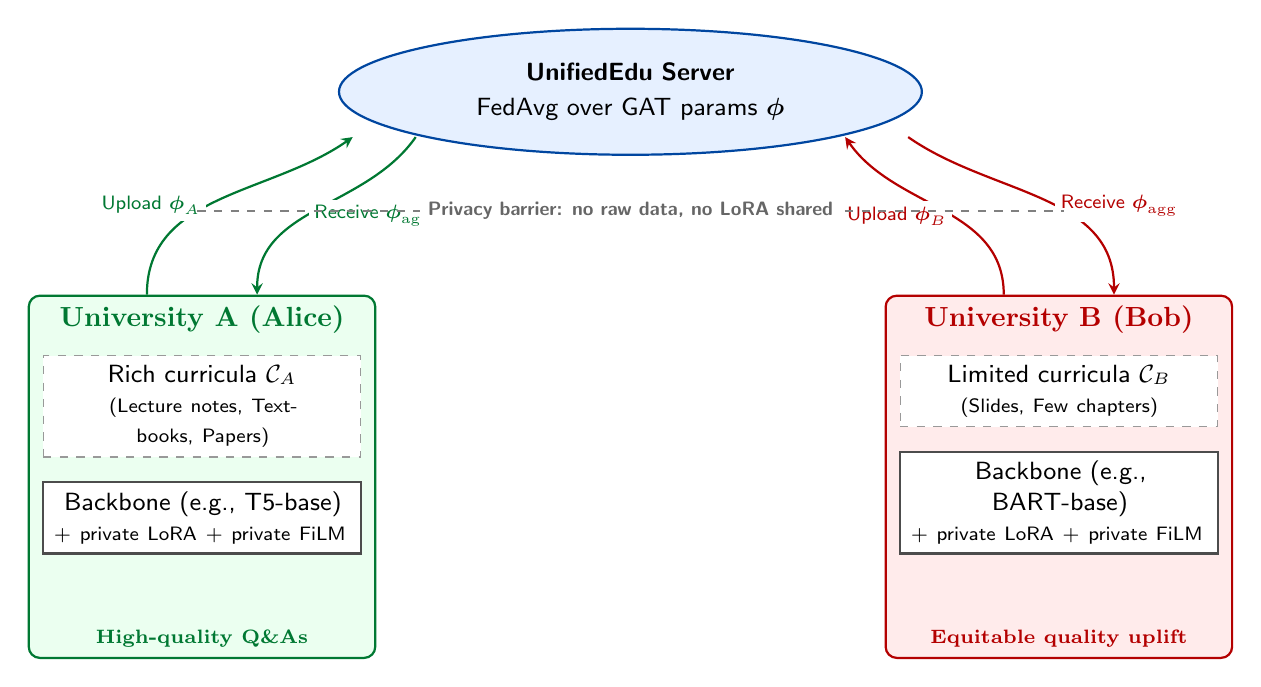
\begin{tikzpicture}[
  >=stealth, font=\sffamily\small,
  server/.style={ellipse, draw=myblue, fill=lightblue,
    thick, text width=5.0cm, align=center,
    minimum height=1.6cm},
  instA/.style={rectangle, rounded corners,
    draw=mygreen, fill=lightgreen, thick,
    minimum width=4.4cm, minimum height=4.6cm},
  instB/.style={rectangle, rounded corners,
    draw=myred, fill=lightred, thick,
    minimum width=4.4cm, minimum height=4.6cm},
  dbox/.style={rectangle, draw=black!40, fill=white,
    dashed, text width=3.8cm, align=center,
    minimum height=0.9cm},
  mbox/.style={rectangle, draw=black!70, fill=white,
    thick, text width=3.8cm, align=center,
    minimum height=0.75cm},
  lbl/.style={fill=white, font=\sffamily\scriptsize,
    inner sep=2pt, align=center}
]
\node[server] (srv)
  {\textbf{\UniEdu{} Server}\\[2pt]
   FedAvg over GAT params $\boldsymbol{\phi}$};

\node[instA, below left=2.0cm and 0.6cm of srv] (A) {};
\node[anchor=north, font=\bfseries\color{mygreen},
      inner sep=4pt] (tA) at (A.north)
  {University A (Alice)};
\node[dbox, below=0.12cm of tA] (dA)
  {Rich curricula $\mathcal{C}_A$\\
   \scriptsize(Lecture notes, Textbooks, Papers)};
\node[mbox, below=0.30cm of dA] (mA)
  {Backbone (e.g., T5-base)\\
   \scriptsize $+$ private LoRA $+$ private FiLM};
\node[anchor=south, font=\scriptsize\bfseries\color{mygreen},
      align=center, inner sep=4pt] at (A.south)
  {High-quality Q\&As};

\node[instB, below right=2.0cm and 0.6cm of srv] (B) {};
\node[anchor=north, font=\bfseries\color{myred},
      inner sep=4pt] (tB) at (B.north)
  {University B (Bob)};
\node[dbox, below=0.12cm of tB] (dB)
  {Limited curricula $\mathcal{C}_B$\\
   \scriptsize(Slides, Few chapters)};
\node[mbox, below=0.30cm of dB] (mB)
  {Backbone (e.g., BART-base)\\
   \scriptsize $+$ private LoRA $+$ private FiLM};
\node[anchor=south, font=\scriptsize\bfseries\color{myred},
      align=center, inner sep=4pt] at (B.south)
  {Equitable quality uplift};

\draw[->, thick, mygreen]
  ([xshift=-0.7cm]A.north)
  to[out=90,in=215]
  node[pos=0.45,left,lbl]{Upload $\boldsymbol{\phi}_A$}
  ([xshift=-0.9cm]srv.south west);
\draw[<-, thick, mygreen]
  ([xshift=0.7cm]A.north)
  to[out=90,in=235]
  node[pos=0.45,right,lbl]{Receive $\boldsymbol{\phi}_{\mathrm{agg}}$}
  ([xshift=-0.1cm]srv.south west);

\draw[->, thick, myred]
  ([xshift=-0.7cm]B.north)
  to[out=90,in=305]
  node[pos=0.45,left,lbl]{Upload $\boldsymbol{\phi}_B$}
  ([xshift=0.1cm]srv.south east);
\draw[<-, thick, myred]
  ([xshift=0.7cm]B.north)
  to[out=90,in=325]
  node[pos=0.45,right,lbl]{Receive $\boldsymbol{\phi}_{\mathrm{agg}}$}
  ([xshift=0.9cm]srv.south east);

\draw[dashed, thick, gray]
  ([xshift=-5.5cm,yshift=-0.7cm]srv.south) --
  ([xshift=5.5cm,yshift=-0.7cm]srv.south)
  node[pos=0.5, fill=white,
       font=\sffamily\scriptsize\bfseries,
       inner sep=3pt, text=black!60]
  {Privacy barrier: no raw data, no LoRA shared};
\end{tikzpicture}
\caption{Overview of the \UniEdu{} framework. Each
institution fine-tunes its own LLM with a private LoRA
adapter and exposes a coarse \emph{architecture graph}
of transformer blocks. A shared GAT encodes each
graph; the GAT parameters $\boldsymbol{\phi}$ are the
only quantity federated. Per-block GAT embeddings drive
a client-local FiLM adapter that residually modulates
the corresponding transformer block's hidden states.
LoRA and FiLM weights, and all curricular data, remain
client-local.}
\label{fig:unifiededu_concept}
\end{figure*}

%% ════════════════════════════════════════════════════════════
\section{The \UniEdu{} Framework}
\label{sec:method}

\subsection{Problem Formulation}
\label{sec:problem}

Consider a federation of $m$ educational institutions
indexed by $k \in [m]$. Each institution $k$ holds a
private dataset $\mathcal{D}_k$ of educational
documents sampled from an institution-specific
distribution $\mathbb{P}_k(c, q, a)$, where $c$ is a
context chunk and $(q, a)$ is a (question, answer)
pair, and where the distributions may differ
substantially across institutions (non-IID).
Institution $k$ deploys a local encoder-decoder
language model $f_k(\cdot;\mathbf{W}_k)$ with
backbone parameters $\mathbf{W}_k \in \mathbb{R}^{d_k}$,
where $d_k$ varies across institutions, and a private
LoRA adapter $\mathbf{L}_k = (\mathbf{A}_k,
\mathbf{B}_k)$ on the attention projections.
Direct aggregation of either $\mathbf{W}_k$ or
$\mathbf{L}_k$ across institutions is impossible
because each has a different dimension and semantic
structure.

The federated objective is to discover shared GAT
parameters $\boldsymbol{\phi}^\star$ such that, used
as the architecture-aware conditioning encoder for
every institution's local model, they minimize the
mean empirical loss across the federation:
\begin{equation}
  \boldsymbol{\phi}^\star
  = \argmin_{\boldsymbol{\phi}}
    \frac{1}{m}\sum_{k=1}^m
    F_k(\boldsymbol{\phi};\,\mathbf{L}_k,
    \boldsymbol{\psi}_k),
  \label{eq:global_objective}
\end{equation}
where $\boldsymbol{\psi}_k$ is the FiLM-adapter
parameters of institution $k$. Both $\mathbf{L}_k$
and $\boldsymbol{\psi}_k$ are kept private and updated
only locally.

\subsection{Architecture Graph}
\label{sec:arch_graph}

Each institution constructs a single coarse
\emph{architecture graph} $\mathcal{G}_k =
(\mathcal{V}_k, \mathcal{E}_k)$ from its local
backbone. The construction is performed once locally
and never leaves the institution.

\begin{itemize}[leftmargin=1.5em, itemsep=2pt]
  \item \textbf{Nodes} $\mathcal{V}_k$: each
  transformer block in the backbone becomes one node.
  For T5, the targets are \texttt{T5Block}; for BART,
  \texttt{BartEncoderLayer} and
  \texttt{BartDecoderLayer}; for LED,
  \texttt{LEDEncoderLayer} and
  \texttt{LEDDecoderLayer}. Embedding and
  language-model head modules are added as additional
  nodes when present.
  \item \textbf{Edges} $\mathcal{E}_k$: directed edges
  connect consecutive blocks in forward-pass order,
  plus a self-loop on every node.
  \item \textbf{Node features} $\mathbf{x}_v \in
  \mathbb{R}^{16}$: a fixed-length feature vector
  encoding (i) layer-type one-hot, (ii) parameter
  count and hidden size in log-scale, (iii) normalized
  depth position within the encoder or decoder stack,
  (iv) encoder/decoder side flag, (v) attention/FFN
  role flag, and (vi) running statistics (mean, std,
  $\ell_2$ norm) of the \emph{effective} weights of
  the block's main projection,
  $\mathbf{W}_{\text{eff}} = \mathbf{W}_{\text{base}}
  + (\alpha/r)\,\mathbf{B}\mathbf{A}$. Statistics
  channels are refreshed every mini-batch so the GAT
  always sees up-to-date LoRA-adjusted summaries.
\end{itemize}

The graph is small (typically $|\mathcal{V}_k| \in
[14, 50]$ depending on backbone size) and admits
efficient batched processing.

\subsection{Shared Graph Attention Encoder}
\label{sec:gnn}

The federated component of \UniEdu{} is a 3-layer
Graph Attention Network~\citep{velickovic2018graph}
$g(\cdot;\boldsymbol{\phi})$ shared by all
institutions:
\begin{itemize}[leftmargin=1.5em, itemsep=1pt]
  \item $\mathrm{GATConv}_1$: $\mathbb{R}^{16}{\to}
  \mathbb{R}^{64}$, 4 heads, concat ($\to
  \mathbb{R}^{256}$);
  \item $\mathrm{GATConv}_2$: $\mathbb{R}^{256}{\to}
  \mathbb{R}^{64}$, 4 heads, concat ($\to
  \mathbb{R}^{256}$);
  \item $\mathrm{GATConv}_3$: $\mathbb{R}^{256}{\to}
  \mathbb{R}^{64}$, 1 head ($\to \mathbb{R}^{64}$).
\end{itemize}
ELU activations and dropout are applied between
layers. Given $\mathcal{G}_k$:
\begin{equation}
  \bigl(\mathbf{Z}_k,\;\mathbf{z}_k^{\text{graph}}\bigr)
  = g(\mathcal{G}_k;\boldsymbol{\phi}),
  \label{eq:gnn_forward}
\end{equation}
with $\mathbf{Z}_k \in \mathbb{R}^{|\mathcal{V}_k|
\times 64}$ and $\mathbf{z}_k^{\text{graph}} =
\mathrm{MeanPool}(\mathbf{Z}_k) \in \mathbb{R}^{64}$.
The GAT runs in FP32 to preserve gradient stability
under mixed-precision LM training.

\subsection{Client-Local FiLM Modulation}
\label{sec:film}

Each institution holds a private FiLM
adapter~\citep{perez2018film} $h(\cdot;
\boldsymbol{\psi}_k)$ that translates per-node GAT
embeddings into block-wise modulators. For each
transformer block $\ell$ with corresponding node
embedding $\mathbf{z}_\ell \in \mathbb{R}^{64}$:
\begin{equation}
  (\boldsymbol{\gamma}_\ell, \boldsymbol{\beta}_\ell)
  = \mathrm{Chunk}\!\left(
      \mathrm{MLP}(\mathbf{z}_\ell;
      \boldsymbol{\psi}_k)
    \right),
  \label{eq:film_mlp}
\end{equation}
where $\boldsymbol{\gamma}_\ell, \boldsymbol{\beta}_\ell
\in \mathbb{R}^{d_{\text{model}}^{(k)}}$, the MLP
has one hidden layer of size 128 with ReLU activation,
and $d_{\text{model}}^{(k)}$ is the hidden dimension
of $k$'s backbone (512 for T5-small, 768 for T5-base /
BART-base / LED-base). Modulation is applied as a
residual hook on the block's output:
\begin{equation}
  \mathbf{H}_\ell \leftarrow \mathbf{H}_\ell
  + \alpha_k \bigl(\boldsymbol{\gamma}_\ell \odot
  \mathbf{H}_\ell + \boldsymbol{\beta}_\ell\bigr),
  \label{eq:film_modulation}
\end{equation}
where $\alpha_k \in \mathbb{R}$ is a learnable scalar
\emph{initialized to zero}, so the adapter is the
identity at the start of training and the modulation
strength is data-driven. The FiLM forward pass is
executed in FP32 with $(\boldsymbol{\gamma},
\boldsymbol{\beta})$ cast to the LM's dtype only at
the modulation step.

\subsection{Local Training Objective}
\label{sec:local_obj}

Every institution fine-tunes for AQAG with a standard
conditional language-modeling loss:
\begin{equation}
  \mathcal{L}_k(\boldsymbol{\phi}, \mathbf{L}_k,
  \boldsymbol{\psi}_k)
  = -\frac{1}{|\mathcal{D}_k|}
  \!\!\sum_{(c,q,a) \in \mathcal{D}_k}\!\!
    \log p_{(\boldsymbol{\phi}, \mathbf{L}_k,
    \boldsymbol{\psi}_k)}(q, a \mid c).
  \label{eq:local_loss}
\end{equation}
$\mathbf{W}_{\text{base}}$ is frozen; gradients flow
to $\boldsymbol{\phi}$, $\mathbf{L}_k$, and
$\boldsymbol{\psi}_k$ jointly through the FiLM hooks.
Optimization uses AdamW with a cosine schedule and
linear warm-up; mini-batches use BF16 autocast on the
LM forward.

\subsection{Federated Optimization}
\label{sec:fed_opt}

\textbf{Round structure.}
At the start of round $t$ the server broadcasts
$\boldsymbol{\phi}^{[t-1]}$. Each institution $k$ runs
its local update loop, producing
$(\boldsymbol{\phi}^{[t]}_{(k)}, \mathbf{L}^{[t]}_k,
\boldsymbol{\psi}^{[t]}_k)$, and uploads
\emph{only} $\boldsymbol{\phi}^{[t]}_{(k)}$. The
LoRA and FiLM updates are stored locally for the next
round and are never transmitted.

\textbf{Server aggregation.}
The server collects
$\{\boldsymbol{\phi}^{[t]}_{(k)}\}_{k=1}^m$ and
performs sample-size-weighted FedAvg
\citep{mcmahan2017communication}:
\begin{equation}
  \boldsymbol{\phi}^{[t]}
  = \sum_{k=1}^m
    \frac{n_k}{\sum_j n_j}\,
    \boldsymbol{\phi}^{[t]}_{(k)},
  \label{eq:fedavg}
\end{equation}
where $n_k = |\mathcal{D}_k^{\text{train}}|$. The
broadcast cost per round is
$\mathcal{O}(|\boldsymbol{\phi}|)$ floats — the GAT
has $\sim$$10^5$ parameters, independent of the
backbone size. LoRA and FiLM are never aggregated, so
heterogeneity in their dimension is irrelevant to the
protocol.

\red{TODO: confirm any client-sampling deviation from
the all-clients-each-round default; verify final round
counts and any warm-up.}

\begin{algorithm}[t]
\caption{\UniEdu{}: unified federated learning for AQAG.}
\label{alg:unifiededu}
\begin{algorithmic}[1]
\Require $m$ institutions; private datasets
  $\{\mathcal{D}_k\}$; private LoRA $\{\mathbf{L}_k\}$;
  private FiLM $\{\boldsymbol{\psi}_k\}$; rounds $T$;
  initial $\boldsymbol{\phi}^{[0]}$; learning rate
  $\eta$.
\Ensure $\boldsymbol{\phi}^{[T]}$ and per-client
  $(\mathbf{L}_k, \boldsymbol{\psi}_k)$.
\For{each institution $k$}
  \State Build $\mathcal{G}_k$ from local backbone (once).
\EndFor
\For{$t = 1,\ldots,T$}
  \State Server broadcasts $\boldsymbol{\phi}^{[t-1]}$.
  \For{each institution $k$ in parallel}
    \For{each local mini-batch
         $(c, q, a) \in \mathcal{D}_k$}
      \State Refresh effective-weight node features.
      \State $(\mathbf{Z}_k, \mathbf{z}_k^{\text{graph}})
             \leftarrow g(\mathcal{G}_k;
             \boldsymbol{\phi})$.
      \State Update FiLM hooks; LM forward + backward.
      \State AdamW step on
             $(\boldsymbol{\phi}, \mathbf{L}_k,
             \boldsymbol{\psi}_k)$.
    \EndFor
    \State Upload
      $\boldsymbol{\phi}^{[t]}_{(k)}$.
  \EndFor
  \State Server: $\boldsymbol{\phi}^{[t]} \leftarrow
         \sum_k \frac{n_k}{\sum_j n_j}
         \boldsymbol{\phi}^{[t]}_{(k)}$.
\EndFor
\State \Return $\boldsymbol{\phi}^{[T]},
       \{(\mathbf{L}_k, \boldsymbol{\psi}_k)\}$.
\end{algorithmic}
\end{algorithm}

%% ════════════════════════════════════════════════════════════
\section{Experimental Setup}
\label{sec:experiments}

We evaluate \UniEdu{} on two complementary testbeds.
The \emph{public testbed}
(\S\ref{sec:public_testbed}) fixes a publicly
reproducible federation built from openly available
ML lecture notes and an arXiv ML paper corpus. It
isolates the effect of architectural heterogeneity
under controlled data conditions and lets external
researchers reproduce the framework end-to-end. The
\emph{private testbed} (\S\ref{sec:private_testbed})
runs the same framework across five real
collaborating institutions training on their own
private curricula, with the sample-size, vocabulary,
and stylistic heterogeneity that real
deployments exhibit.

For both testbeds we share the same model zoo
(\S\ref{sec:models}), training procedure
(\S\ref{sec:training}), baselines
(\S\ref{sec:baselines}), and evaluation suite
(\S\ref{sec:evaluation}). We report results on val
splits (\S\ref{sec:results}); test splits are held
out for cross-testbed comparisons in future work.

\subsection{Public Testbed: Open ML Curricula}
\label{sec:public_testbed}

The public testbed comprises three institutions
$(\mathcal{I}_0, \mathcal{I}_1, \mathcal{I}_2)$ whose
curricula are constructed from openly available
sources, so the entire pipeline can be reproduced by
anyone with the corresponding files. The three
sources are:
\begin{itemize}[leftmargin=1.5em, itemsep=2pt]
  \item $\mathcal{I}_0$: \textbf{MIT 18.657 ---
  Mathematics of Machine
  Learning}~\citep{mit18657}, lecture notes covering
  statistical learning theory and optimisation. 110
  context chunks, 547 GPT-4o-annotated QA pairs.
  \item $\mathcal{I}_1$: \textbf{Stanford
  CS229}~\citep{stanfordcs229}, undergraduate ML
  course notes covering supervised and unsupervised
  learning, neural networks, and reinforcement
  learning. 110 context chunks, 559 GPT-4o-annotated
  QA pairs.
  \item $\mathcal{I}_2$: \textbf{ML papers
  (arXiv)}, a curated set of recent machine-learning
  preprints across vision, NLP, and reinforcement
  learning. 981 context chunks, 5{,}037
  GPT-4o-annotated QA pairs.
\end{itemize}

\textbf{Data preparation.}
Source PDFs are converted to plain-text chunks of
150--400 words each (one coherent topic per chunk,
boilerplate and figure captions stripped). For every
chunk we generate exactly five (question, answer)
pairs with GPT-4o, each labelled with its
\texttt{question\_topic} (a 2--4-word ML concept
phrase), Bloom's Revised Taxonomy level
(integer 1--6), difficulty
(\texttt{easy}/\texttt{medium}/\texttt{hard}), and
an \texttt{answerable\_from\_context} flag. JSON
outputs are validated against a schema before
splitting.

\textbf{Splits.}
Splits are at the chunk level (not at the QA-pair
level) to prevent context leakage. Each institution
holds out 15\% of chunks as a fixed test set and
divides the remaining 85\% into three equal CV folds.
The split seed is 42 across all collaborators so that
splits are bit-for-bit reproducible. We provide the
checksums (Appendix~\ref{app:reproducibility}) to
allow third-party verification.

\textbf{Heterogeneity.} Sample sizes differ by an order
of magnitude across the public testbed
($\mathcal{I}_0,\mathcal{I}_1$: $\sim$110 chunks;
$\mathcal{I}_2$: 981 chunks), giving a controlled
non-IID setting. We additionally report a
\emph{balanced} variant of the public testbed in which
$\mathcal{I}_2$ is sub-sampled to 110 chunks; the
contrast between balanced and unbalanced runs probes
whether \UniEdu{}'s federation gain is an artefact of
data quantity or of the GAT-mediated transfer
(Appendix~\ref{app:balanced_vs_unbalanced}).

\subsection{Private Testbed: Real-World Federation}
\label{sec:private_testbed}

The private testbed instantiates \UniEdu{} across
\textbf{five real collaborating institutions} that
each contribute their own private machine-learning
curricula. Concretely, each collaborator
(i)~runs the Phase~1 data-preparation pipeline locally
on their own materials (PDF lectures, PPTX decks,
research papers), producing a JSON file conforming to
the same schema as the public testbed; (ii)~validates
their file with our schema validator; (iii)~generates
deterministic 3-fold CV splits with the shared seed
$=42$; and (iv)~ships only the resulting checksum
file to the coordinator for cross-collaborator
reproducibility verification. \emph{No raw
curricular data, no QA pairs, and no model weights
ever cross institutional boundaries.}

The five institutions are assigned different SLM
backbones based on declared GPU resources and
software preferences (Table~\ref{tab:client_models}),
prioritising architectural diversity. The federation
involves no central training corpus; each
institution's training data is its own.
\red{TODO: institutional names (or anonymous IDs
$\mathcal{I}_0,\dots,\mathcal{I}_4$); recruitment-form
demographic figure; per-institution chunk and QA-pair
counts; topic-coverage histograms.}

\subsection{Model Zoo}
\label{sec:models}

Across both testbeds, the SLMs span five
encoder-decoder families with different attention
mechanisms, pre-training objectives, and effective
context windows (Table~\ref{tab:client_models}).

\begin{table}[t]
\centering
\small
\caption{SLMs used in the public and private testbeds.
LoRA targets follow each model family's attention
projection naming. $d_{\text{model}}$ is the hidden
size, used for the FiLM modulator in
Eq.~\ref{eq:film_mlp}.}
\label{tab:client_models}
\begin{tabular}{lll@{\hskip 4pt}lr}
\toprule
\textbf{Backbone} & \textbf{Family} &
\textbf{LoRA targets} & \textbf{$d_{\text{model}}$} &
\textbf{Params} \\
\midrule
BART-base                & \texttt{bart}       & \texttt{q\_proj v\_proj}        & 768 & 140M \\
Flan-T5-base             & \texttt{t5}         & \texttt{q v}                    & 768 & 250M \\
LED-base-16384           & \texttt{led}        & \texttt{q\_proj v\_proj}        & 768 & 162M \\
Pegasus-X-base           & \texttt{pegasus\_x} & \texttt{q\_proj v\_proj}        & 768 & 272M \\
ProphetNet-large         & \texttt{prophetnet} & \texttt{query\_proj value\_proj} & 1024 & 392M \\
\bottomrule
\end{tabular}
\end{table}

\subsection{Training Procedure}
\label{sec:training}

\textbf{Per-fold local training.} Each institution
trains its SLM with its private LoRA adapter for up
to 100 epochs with early stopping on a fast
generation-based metric (greedy-decoded ROUGE-L on a
fixed 50-sample val subsample), patience 10
($\Delta_{\min}{=}10^{-4}$), and saves both the
\emph{best} (lowest val-loss) and \emph{final}
(last-epoch) LoRA checkpoints for separate evaluation.

\textbf{Local optimisation.} AdamW with peak learning
rate $3{\times}10^{-4}$, cosine schedule with 10\%
linear warm-up, gradient clipping 1.0, batch size 4,
LoRA rank $r{=}16$ and $\alpha{=}32$, LoRA dropout
$0.1$, mixed-precision BF16 autocast on the LM
forward.

\textbf{Conditioning regimes.} Each institution
trains its SLM under three prompt-conditioning
regimes (\S\ref{sec:conditioning}): \texttt{baseline}
(context only, with diverse beam search and
Hungarian-matched references at evaluation),
\texttt{topic} (prompt embeds the QA's
\texttt{question\_topic}), and \texttt{bloom} (prompt
embeds the QA's Bloom level and corresponding
cognitive verb). All three are evaluated separately;
the comparisons in \S\ref{sec:results} use
\texttt{topic} unless otherwise stated.

\textbf{Federated optimisation.} \UniEdu{} runs $T=33$
federation rounds with $3$ local epochs per round and
sample-size-weighted FedAvg of the GAT parameters
$\boldsymbol{\phi}$ (\S\ref{sec:fed_opt}). The total
effective passes per client $\approx 99$, comparable
to the individual baseline. We use a single best-
checkpoint snapshot at the round with the lowest
average val loss across clients to align with the
individual baseline's early-stopping protocol.

\subsection{Conditioning Regimes}
\label{sec:conditioning}

To address the duplicate-QA pathology that arises
when many QA pairs share a context, the prompt seen
by the SLM at training and inference time can be
conditioned on additional fields:
\begin{itemize}[leftmargin=1.5em, itemsep=2pt]
  \item \texttt{baseline}: ``\textit{Generate a
  question and answer pair from the following machine
  learning text:} {[}context{]}''. At evaluation,
  diverse beam search produces five generations per
  unique context, then Hungarian-matched to the
  context's five reference QA pairs via ROUGE-L.
  \item \texttt{topic}: ``\textit{Generate a question
  and answer pair about }``{[}topic{]}''\textit{
  from the following machine learning text:}
  {[}context{]}''. Each input is unique, so standard
  beam search is used at evaluation.
  \item \texttt{bloom}: ``\textit{Generate a Bloom
  Level-{[}b{]} ({[}verb{]}) question and answer pair
  from the following machine learning text:}
  {[}context{]}'', where \texttt{[verb]} is the
  cognitive verb anchored at level $b$
  (Remember/Understand/Apply/Analyse/Evaluate/Create).
\end{itemize}

\subsection{Baselines}
\label{sec:baselines}

The two hypotheses in \S\ref{sec:scenario} require
distinct sets of comparators.

\paragraph{For H1 (equity).}
We compare \UniEdu{} against \emph{federation-level}
methods that, like \UniEdu{}, assume a federation of
SLMs and evaluate per-institution QA quality on
the same val set:
\begin{itemize}[leftmargin=1.5em, itemsep=2pt]
  \item \textbf{Indiv} (lower bound). Each
  institution trains its SLM with a private LoRA
  adapter on its own data, with no federation. Three
  conditioning regimes per institution
  (\S\ref{sec:conditioning}).
  \item \textbf{FedKD}~\citep{wu2022fedkd}.
  Communication-efficient federated learning via
  knowledge distillation: each client trains a small
  ``mentee'' model that distils both the local
  ``mentor'' and the federated ensemble; only mentee
  parameters are exchanged. \red{TODO: implement
  FedKD in \texttt{unifiedfl/}.}
  \item \textbf{FedMD}~\citep{li2019fedmd}. The
  canonical heterogeneous-federated-learning
  baseline. Each client trains its own SLM locally,
  then communicates predictions on a shared
  public dataset; the server aggregates predictions
  into a consensus, and clients distil that consensus
  back into their local SLM. Architectural
  heterogeneity is handled by-design because clients
  exchange logits rather than parameters. We use the
  public-testbed chunks (\S\ref{sec:public_testbed})
  as the shared dataset. \red{TODO: implement FedMD
  in \texttt{unifiedfl/}.}
  \item \textbf{FedDF}~\citep{lin2020feddf}.
  Server-side ensemble distillation on an unlabelled
  public dataset; no parameter averaging. Like
  FedMD, accommodates heterogeneous SLMs through
  output-space rather than parameter-space exchange,
  but moves the distillation step to the server.
  Re-uses the same public dataset as FedMD.
  \red{TODO: implement FedDF in \texttt{unifiedfl/}.}
  \item \textbf{FedET}~\citep{cheng2022fedet}.
  Communicates per-client embeddings rather than
  logits: each client uploads its hidden-state
  representations on the shared public dataset, the
  server fuses them via a small enhanced-transformer
  aggregator, and clients distil the fused
  representation back into their local SLM. Closer
  in spirit to \UniEdu{}'s embedding-channel design
  than FedMD/FedDF's logit channel. \red{TODO:
  implement FedET in \texttt{unifiedfl/}.}

\smallskip
Implementation details for all four
distillation-based baselines (mentor/mentee setup,
distillation losses, hyperparameters,
public-dataset usage) are in
Appendix~\ref{app:baseline_implementations}.
  \item \textbf{\UniEdu{}-static} (ablation):
  architecture-graph features fixed at round~0, no
  per-batch refresh of effective-weight statistics.
  Ablates the dynamic feature update.
  \item \textbf{\UniEdu{}-noFiLM} (ablation):
  GAT trained but its embeddings unused at the LM
  forward. Ablates the conditioning channel.
  \item \textbf{\UniEdu{}} (full): GAT-FedAvg, LoRA
  and FiLM client-local, per-batch effective-weight
  refresh.
\end{itemize}

\paragraph{For H2 (LLM approximation).}
We compare the federated mixture of all SLMs ---
i.e., \UniEdu{} aggregated across institutions, not
each institution in isolation --- against
single-model LLMs prompted zero-shot to produce a
$(q, a)$ pair from each test context, run through
the same evaluation suite:
\begin{itemize}[leftmargin=1.5em, itemsep=2pt]
  \item \textbf{GPT-4o} \red{(headline ceiling)}.
  \item \textbf{GPT-4o-mini}.
  \item \textbf{Llama-3.1-8B-Instruct}~\citep{grattafiori2024llama3}.
  \item \textbf{Qwen-2.5-7B-Instruct}~\citep{bai2023qwen}.
  \item \textbf{Mistral-7B-Instruct}~\citep{jiang2023mistral}.
  \item \textbf{Gemini-1.5-Flash}.
\end{itemize}
The H2 panel is reported separately
(\S\ref{sec:results_llm_approx},
Appendix~\ref{app:llm_baselines}); these LLMs do not
appear as rows in the per-institution H1 tables.

\subsection{Hyperparameters}
\label{sec:hyperparams}

The full hyperparameter table is in
Appendix~\ref{app:hyperparams}. Defaults are: AdamW
peak LR $3{\times}10^{-4}$ with 10\% cosine warm-up;
gradient clipping 1.0; batch size 4;
$\texttt{max\_input\_len}{=}512$;
$\texttt{max\_target\_len}{=}128$; LoRA $r{=}16$,
$\alpha{=}32$, dropout $0.1$; FiLM hidden 128,
$\alpha_{\text{init}}{=}0$; GAT 3 layers, 4 heads,
hidden 64, dropout $0.1$; federation $T{=}33$ rounds
with 3 local epochs per round; individual training
up to $100$ epochs with patience $10$ on greedy-ROUGE-L
over a fixed 50-sample val subsample.

%% ════════════════════════════════════════════════════════════
\section{Evaluation Framework}
\label{sec:evaluation}

For a given source context $c$ and a generated
question-answer pair $(q, a)$, the framework evaluates
six orthogonal dimensions of quality
(Table~\ref{tab:eval_overview}).

\begin{table}[t]
\centering
\small
\caption{Evaluation dimensions for \UniEdu{}.}
\label{tab:eval_overview}
\begin{tabular}{p{2.0cm}p{4.6cm}}
\toprule
\textbf{Dimension} & \textbf{Metric(s)} \\
\midrule
Question quality & RQUGE \citep{mohammadshahi2023rquge} \\
Answer quality   & RAGAS Faithfulness \citep{es2023ragas};
                   QAFactEval \citep{fabbri2022qafacteval} \\
Joint QA quality & RTC \citep{alberti2019synthetic};
                   RAGAS Answer Relevancy
                   \citep{es2023ragas} \\
Pedagogical      & Bloom's BERT classifier; Bloom's LLM
                   judge; EVS \\
QA-quality LLM judge
                 & Four-dimension GPT-4o rubric
                   (context grounding, educational
                   value, answer correctness, answer
                   relevance) \\
Equity           & Pairwise Equity; Knowledge Transfer
                   Index; Anchor Question Equity \\
\bottomrule
\end{tabular}
\end{table}

\subsection{Question Quality: RQUGE}
\label{sec:rquge}

\textbf{RQUGE}~\citep{mohammadshahi2023rquge} is a
reference-free metric that scores question quality
through answerability. Given context $c$, candidate
question $q$, and gold answer span $a_r$ (the
generated $a$):
\begin{equation}
  a_c = \mathrm{QA}(q, c),\qquad
  \kappa = S(q, a_c, a_r, c),
  \label{eq:rquge}
\end{equation}
where $\mathrm{QA}(\cdot)$ is
UnifiedQA-v2~\citep{khashabi2022unifiedqa} and
$S(\cdot)$ is a span-quality scorer; $\kappa \in [1,
5]$. We use a BERTScore-based approximation of
$S(\cdot)$, scaled to $[1, 5]$ via $\kappa = 1 + 4
\cdot \mathrm{BERTScore\text{-}F1}$ (clamped).

\subsection{Answer Quality}
\label{sec:answer_quality}

\textbf{RAGAS Faithfulness}~\citep{es2023ragas}
decomposes $a$ into atomic claims $\mathcal{S}(a)$
(by NLTK sentence splitting, or by a GPT-4o-mini
decomposer when an OpenAI key is provided) and
verifies each claim with an NLI
model~\citep{he2021deberta}:
\begin{equation}
  \mathrm{Faithfulness}(a, c)
  = \frac{1}{|\mathcal{S}(a)|}\!
    \sum_i \mathbf{1}[\mathrm{NLI}(c, s_i){=}\texttt{ENT}].
  \label{eq:faithfulness}
\end{equation}

\textbf{QAFactEval}~\citep{fabbri2022qafacteval} is
approximated via UnifiedQA: each sentence-level claim
is wrapped in a yes/no probe answered against $c$;
the score is the mean ``yes'' rate.

\subsection{Joint Question-Answer Quality}
\label{sec:joint_quality}

\textbf{Round-Trip Consistency (RTC)}, inspired by
\citet{alberti2019synthetic}:
\begin{equation}
  \mathrm{RTC}(q, a, c)
  = \mathrm{F1}_{\text{tok}}\!\left(
      \mathrm{QA}(q, c), a
    \right).
  \label{eq:rtc}
\end{equation}
We use token-level F1 (rather than the original
exact-match) for a continuous score suitable for
cross-paradigm comparison.

\textbf{RAGAS Answer Relevancy}~\citep{es2023ragas}
generates $n$ reverse questions $\{\hat{q}_i\}$ from
$a$ and computes:
\begin{equation}
  \mathrm{AR}(q, a) =
  \tfrac{1}{n}\!\sum_{i=1}^{n}
    \frac{\mathbf{e}_q^{\!\top}\mathbf{e}_{\hat{q}_i}}
         {\|\mathbf{e}_q\|\,\|\mathbf{e}_{\hat{q}_i}\|}.
  \label{eq:answer_relevancy}
\end{equation}

\subsection{Pedagogical Quality}
\label{sec:pedagogical}

We adopt \textbf{Bloom's Revised
Taxonomy}~\citep{anderson2001taxonomy} (six levels:
Remember, Understand, Apply, Analyze, Evaluate,
Create) and assess cognitive depth via two
independent classifiers:

\textbf{Bloom's BERT classifier.} A publicly
available BERT-base classifier
(\texttt{cip29/bert-blooms-taxonomy-classifier})
fine-tuned on Bloom's-labeled question data:
\begin{equation}
  \hat{b}(q) = \argmax_{b}\,
    \mathrm{softmax}(W \cdot \mathrm{BERT}(q))_b.
  \label{eq:bloom_bert}
\end{equation}

\textbf{Bloom's LLM judge.} GPT-4o-mini queried with
a structured prompt that supplies the six levels with
verb-anchored definitions and asks for a JSON output
$\{\texttt{level}, \texttt{reason}\}$.

The Bloom's level is normalized to a continuous
\textbf{Educational Value Score}:
\begin{equation}
  \mathrm{EVS}(q) = \tfrac{\hat{b}(q) - 1}{5}
  \in [0, 1].
  \label{eq:evs}
\end{equation}

\subsection{LLM QA-Quality Judge}
\label{sec:llm_judge}

A four-dimension LLM judge (GPT-4o, JSON-object output)
rates each $(c, q, a)$ on a strict 1--5 rubric for
\emph{context grounding}, \emph{educational value},
\emph{answer correctness}, and \emph{answer relevance},
with verb-anchored anchors at levels 1, 3, 5
(prompt in Appendix~\ref{app:llm_judge_prompt}).
Aggregated overall $\in [0, 1]$ via
$(\bar{s} - 1)/4$.

\subsection{Equity Evaluation}
\label{sec:equity}

Let $m \in \{\indiv, \fed, \uni\}$ denote the
learning paradigm. $Q_k^{(m)}$ is institution $k$'s
aggregate quality (default: LLM-judge overall);
$\mathcal{C}_k$ its curricular richness;
$\mathcal{R}_k$ its compute resource (trainable
parameter count of the deployed backbone, normalized
by the largest in the federation).

\subsubsection{Pairwise Equity Score}
\label{sec:pairwise_equity}

\begin{definition}[Pairwise Equity Score]
\begin{equation}
  E_{kl}^{(m)}
  = \frac{Q_k^{(m)} + Q_l^{(m)}}
         {|\mathcal{C}_k - \mathcal{C}_l|
          + |\mathcal{R}_k - \mathcal{R}_l| + \varepsilon},
  \label{eq:pairwise_equity}
\end{equation}
where $\varepsilon{=}10^{-6}$ stabilizes the
denominator when resources are nearly matched.
\end{definition}

\begin{remark}
A high $E_{kl}^{(m)}$ rewards configurations in
which both institutions benefit \emph{simultaneously},
not configurations that close the gap by degrading
the stronger institution.
\end{remark}

The central hypothesis predicts:
\begin{equation}
  \boxed{E_{kl}^{(\uni)} > E_{kl}^{(\fed)} >
         E_{kl}^{(\indiv)}}
  \label{eq:equity_ordering}
\end{equation}
where $(\fed)$ is well-defined only for
same-architecture pairs; for cross-architecture pairs
the ordering reduces to $E_{kl}^{(\uni)} >
E_{kl}^{(\indiv)}$.

\subsubsection{Anchor Question Equity Score}
\label{sec:anchor_equity}

\begin{definition}[Anchor Question Setup]
Let $q^*$ be a fixed anchor question covering a core
ML concept. Consider $k, l$ with
\begin{equation}
  \mathcal{C}_k > \mathcal{C}_l,\qquad
  \mathcal{R}_k = \mathcal{R}_l.
  \label{eq:anchor_condition}
\end{equation}
\end{definition}

An LLM Equity Judge (constrained-rubric GPT-4o)
scores each model's response to $q^*$:
$s_k^{(\indiv)}$, $s_l^{(\indiv)}$, $s_l^{(\uni)}
\in [0, 1]$.

\begin{proposition}[Anchor Equity Hypothesis]
Under Eq.~\ref{eq:anchor_condition}:
\begin{equation}
  \boxed{s_l^{(\uni)} \approx s_k^{(\indiv)} >
         s_l^{(\indiv)}}
  \label{eq:anchor_hypothesis}
\end{equation}
\end{proposition}

\red{TODO: confirm at least one collaborator pair
satisfies Eq.~\ref{eq:anchor_condition}, or
operationalize an approximate matching by binning
$\mathcal{R}_k$.}

\subsubsection{Knowledge Transfer Index}
\label{sec:kti}

To distinguish knowledge transfer from regularization:
\begin{equation}
  \mathrm{KTI}(l \leftarrow k)
  = Q_l^{(\uni)}(\mathcal{T}_{k\setminus l})
  - Q_l^{(\indiv)}(\mathcal{T}_{k\setminus l}),
  \label{eq:kti}
\end{equation}
where $\mathcal{T}_{k\setminus l}$ is a held-out test
set covering topics exclusive to $k$'s curriculum.
A positive KTI on these items provides direct
evidence of cross-institutional transfer rather than a
regularization artifact of GAT averaging. The
\textbf{\UniEdu{}-noFiLM} ablation
(§\ref{sec:baselines}) is the natural control: if
KTI persists in full \UniEdu{} but vanishes in
\UniEdu{}-noFiLM, the conditioning channel carries
the cross-client knowledge.

\subsection{Statistical Validation}
\label{sec:stats}

For each institution $k$ and each metric $Q$, we
collect per-sample score vectors
$\mathcal{D}_k^{(\indiv)}$ and $\mathcal{D}_k^{(\uni)}$
from val-set evaluation under each paradigm. We apply
a one-sided \textbf{paired Wilcoxon signed-rank test}
(preferred over the paired $t$-test, since NLP
quality scores are typically non-Gaussian and bounded):
\begin{equation}
  H_0: \mu_{Q^{(\uni)}} = \mu_{Q^{(\indiv)}},\quad
  H_1: \mu_{Q^{(\uni)}} > \mu_{Q^{(\indiv)}}.
  \label{eq:hypothesis_test}
\end{equation}
We report $p$-values at $\alpha{=}0.05$ with
\textbf{Bonferroni correction} across the (metric,
institution) grid, \textbf{Cohen's} $d$ for effect
size, and \textbf{95\,\% bootstrap CIs}
($B{=}10{,}000$).

%% ════════════════════════════════════════════════════════════
\section{Results}
\label{sec:results}

The two hypotheses (\S\ref{sec:scenario}) are
reported separately. \S\ref{sec:results_equity} and
\S\ref{sec:results_kti} test \textbf{H1} (equity)
by comparing \UniEdu{} against per-institution local
training. The result for the equity story is
\emph{per-institution}; GPT-4o does not appear as a
row. \S\ref{sec:results_llm_approx} tests
\textbf{H2} (LLM approximation) by aggregating
\UniEdu{}'s output across the federation and
comparing the aggregate against single-LLM zero-shot
baselines. For the public testbed we evaluate on
three slices: each client's local val set (held out
during training and used for early stopping), each
client's local test set (held out from training,
in-distribution), and an
$\mathcal{T}^{\text{global}}$ pool of $916$
held-out chunks aggregated across all three clients
(cross-distribution). All metrics are reported as
the mean over 3-fold cross-validation. We report
both the BEST checkpoint (selected on val ROUGE-L)
and the FINAL checkpoint at the last completed
epoch / round; the appendix
(\S\ref{app:final_ckpt}) holds the FINAL-checkpoint
counterparts of every main-paper table. Score
directions: ROUGE-L / BLEU-4 / BERTScore-F1 / RTC /
Faithfulness / QAFactEval / Answer-Relevancy /
Bloom-EVS / LLM-judge overall are all
higher-is-better in $[0, 1]$. RQUGE is
higher-is-better in $[1, 5]$. The Pairwise Equity
Score $\bar{E}$ (Eq.~\ref{eq:pairwise_equity}) is
higher-is-better and unbounded above.

\subsection{H1 — Equity Comparison}
\label{sec:results_equity}

We compare \UniEdu{} (architecture-aware federated
LoRA + FiLM, \S\ref{sec:framework}) against the
per-institution local baseline \textbf{Indiv} on the
public testbed (Table~\ref{tab:headline_global},
Table~\ref{tab:val_test}). Federation lifts every
lightweight metric over the individual baseline on
the cross-distribution global test set: ROUGE-L
improves by $+0.0087$, BLEU-4 by $+0.0119$,
BERTScore-F1 by $+0.0040$, and the local Bloom's
educational-value score by $+0.0041$ (mean across
the three institutions, best checkpoint;
Table~\ref{tab:headline_global}). The gain is
largest for $\mathcal{I}_2$ (LED-16384, ML papers)
--- the smallest-data, most under-represented
institution --- where federation improves all four
lightweight metrics simultaneously by margins of
$+0.0166$ / $+0.0201$ / $+0.0058$ / $+0.0304$. On
each client's own local test
(Table~\ref{tab:val_test}, lower half), the
individual baseline retains its specialisation
advantage on the native distribution: Indiv wins
ROUGE-L on $\mathcal{I}_0$ and $\mathcal{I}_1$.
\UniEdu{}, however, still wins all four lightweight
metrics on $\mathcal{I}_2$'s local test --- the
federation's value is most pronounced exactly where
local data is scarcest. Cross-architecture
federation across BART, Flan-T5, and LED
simultaneously, a setting prior heterogeneous-FL
work~\citep{wu2022fedkd, li2019fedmd, lin2020feddf,
cheng2022fedet} did not attempt, is therefore not a
breadth tax but the very mechanism that levels the
playing field for the data-poor client.

% TODO(fp): re-run all (client, fold) cells with --no-heavy off + an
% OpenAI key to populate the LLM-based block (RTC, Faith., QAFE, RQUGE,
% Ans-Rel, Bloom-LLM EVS, LLM-judge overall). The current --fast-eval
% pass produced only the four lightweight columns.
\begin{table*}[t]
\centering
\footnotesize
\setlength{\tabcolsep}{2pt}
\caption{H1 headline: \UniEdu{} vs the per-institution
individual baseline (\textbf{Indiv}) on the
cross-distribution \textbf{global test set}
($\mathcal{T}^{\text{global}}$, $916$ samples
pooled across institutions; best checkpoint, mean
over 3 folds). Lightweight reference-based metrics
on the left; reference-free LLM-based metrics on
the right (\S\ref{sec:eval}). Bold = better of
$\{\indiv, \uni\}$ per (institution, metric).}
\label{tab:headline_global}
\begin{tabular}{ll cccc ccccccc}
\toprule
\multirow{2}{*}{\textbf{Inst.}} &
\multirow{2}{*}{\textbf{Method}} &
\multicolumn{4}{c}{\textbf{Lightweight}} &
\multicolumn{7}{c}{\textbf{LLM-based / reference-free}} \\
\cmidrule(lr){3-6} \cmidrule(lr){7-13}
& &
\textbf{R-L} & \textbf{B-4} & \textbf{BERT} & \textbf{B\textsubscript{cls}} &
\textbf{B\textsubscript{LLM}} & \textbf{AnsR} & \textbf{Faith} & \textbf{QAFE} &
\textbf{RQU} & \textbf{RTC} & \textbf{LLM-J} \\
\midrule
\multirow{2}{*}{$\mathcal{I}_0$ (BART, MIT)}
  & \indiv     & 0.4290 & 0.1610 & 0.8595 & \textbf{0.2400} & --- & --- & --- & --- & --- & --- & --- \\
  & \UniEdu{}  & \textbf{0.4322} & \textbf{0.1653} & \textbf{0.8604} & 0.2164 & --- & --- & --- & --- & --- & --- & --- \\
\midrule
\multirow{2}{*}{$\mathcal{I}_1$ (Flan-T5, Stanford)}
  & \indiv     & 0.4422 & 0.1646 & 0.8623 & 0.2705 & --- & --- & --- & --- & --- & --- & --- \\
  & \UniEdu{}  & \textbf{0.4483} & \textbf{0.1759} & \textbf{0.8675} & \textbf{0.2758} & --- & --- & --- & --- & --- & --- & --- \\
\midrule
\multirow{2}{*}{$\mathcal{I}_2$ (LED, ML papers)}
  & \indiv     & 0.4246 & 0.1595 & 0.8592 & 0.1627 & --- & --- & --- & --- & --- & --- & --- \\
  & \UniEdu{}  & \textbf{0.4412} & \textbf{0.1796} & \textbf{0.8650} & \textbf{0.1932} & --- & --- & --- & --- & --- & --- & --- \\
\midrule
\multirow{2}{*}{Mean across $\mathcal{I}_{0,1,2}$}
  & \indiv     & 0.4319 & 0.1617 & 0.8603 & 0.2244 & --- & --- & --- & --- & --- & --- & --- \\
  & \UniEdu{}  & \textbf{0.4406} & \textbf{0.1736} & \textbf{0.8643} & \textbf{0.2284} & --- & --- & --- & --- & --- & --- & --- \\
\bottomrule
\end{tabular}
\end{table*}

% TODO(fp): same back-fill applies — local val and local test cells
% currently populated for lightweight metrics only.
\begin{table*}[t]
\centering
\footnotesize
\setlength{\tabcolsep}{2pt}
\caption{In-distribution comparison on the public
testbed (best checkpoint, mean over 3 folds). Top
half: each client's \textbf{local val} set; bottom
half: each client's \textbf{local test} set. Bold =
better of $\{\indiv, \uni\}$ per (institution,
metric).}
\label{tab:val_test}
\begin{tabular}{ll cccc ccccccc}
\toprule
\multirow{2}{*}{\textbf{Inst.}} &
\multirow{2}{*}{\textbf{Method}} &
\multicolumn{4}{c}{\textbf{Lightweight}} &
\multicolumn{7}{c}{\textbf{LLM-based / reference-free}} \\
\cmidrule(lr){3-6} \cmidrule(lr){7-13}
& &
\textbf{R-L} & \textbf{B-4} & \textbf{BERT} & \textbf{B\textsubscript{cls}} &
\textbf{B\textsubscript{LLM}} & \textbf{AnsR} & \textbf{Faith} & \textbf{QAFE} &
\textbf{RQU} & \textbf{RTC} & \textbf{LLM-J} \\
\midrule
\multicolumn{13}{l}{\textit{Local val (per client)}} \\
\midrule
\multirow{2}{*}{$\mathcal{I}_0$}
  & \indiv     & 0.4778 & 0.1951 & 0.8762 & \textbf{0.2088} & --- & --- & --- & --- & --- & --- & --- \\
  & \UniEdu{}  & \textbf{0.4838} & \textbf{0.2052} & \textbf{0.8799} & 0.1928 & --- & --- & --- & --- & --- & --- & --- \\
\multirow{2}{*}{$\mathcal{I}_1$}
  & \indiv     & 0.4851 & 0.1868 & 0.8720 & 0.2369 & --- & --- & --- & --- & --- & --- & --- \\
  & \UniEdu{}  & \textbf{0.4880} & \textbf{0.2019} & \textbf{0.8810} & \textbf{0.2524} & --- & --- & --- & --- & --- & --- & --- \\
\multirow{2}{*}{$\mathcal{I}_2$}
  & \indiv     & 0.4253 & 0.1603 & 0.8589 & 0.1737 & --- & --- & --- & --- & --- & --- & --- \\
  & \UniEdu{}  & \textbf{0.4405} & \textbf{0.1789} & \textbf{0.8642} & \textbf{0.2088} & --- & --- & --- & --- & --- & --- & --- \\
\multirow{2}{*}{Mean}
  & \indiv     & 0.4627 & 0.1807 & 0.8691 & 0.2064 & --- & --- & --- & --- & --- & --- & --- \\
  & \UniEdu{}  & \textbf{0.4708} & \textbf{0.1953} & \textbf{0.8750} & \textbf{0.2180} & --- & --- & --- & --- & --- & --- & --- \\
\midrule
\multicolumn{13}{l}{\textit{Local test (per client)}} \\
\midrule
\multirow{2}{*}{$\mathcal{I}_0$}
  & \indiv     & \textbf{0.4793} & \textbf{0.2019} & \textbf{0.8764} & \textbf{0.2042} & --- & --- & --- & --- & --- & --- & --- \\
  & \UniEdu{}  & 0.4547 & 0.1679 & 0.8704 & 0.1353 & --- & --- & --- & --- & --- & --- & --- \\
\multirow{2}{*}{$\mathcal{I}_1$}
  & \indiv     & \textbf{0.4799} & \textbf{0.1829} & 0.8689 & 0.2173 & --- & --- & --- & --- & --- & --- & --- \\
  & \UniEdu{}  & 0.4483 & 0.1685 & \textbf{0.8725} & \textbf{0.2576} & --- & --- & --- & --- & --- & --- & --- \\
\multirow{2}{*}{$\mathcal{I}_2$}
  & \indiv     & 0.4206 & 0.1565 & 0.8579 & 0.1717 & --- & --- & --- & --- & --- & --- & --- \\
  & \UniEdu{}  & \textbf{0.4270} & \textbf{0.1612} & \textbf{0.8604} & \textbf{0.1812} & --- & --- & --- & --- & --- & --- & --- \\
\multirow{2}{*}{Mean}
  & \indiv     & \textbf{0.4599} & \textbf{0.1804} & 0.8677 & \textbf{0.1977} & --- & --- & --- & --- & --- & --- & --- \\
  & \UniEdu{}  & 0.4433 & 0.1658 & \textbf{0.8678} & 0.1914 & --- & --- & --- & --- & --- & --- & --- \\
\bottomrule
\end{tabular}
\end{table*}

% TODO(fp): private testbed (5 institutions) not yet collected; cells stay
% as "--" until Phase~2 of the private collaboration finishes. Methods rows
% (FedKD/MD/DF/ET) are also TODO — those baselines have not been run yet
% on the public testbed either.
\begin{table*}[t]
\centering
\small
\caption{Equity comparison on the \textbf{private
testbed} (\S\ref{sec:private_testbed}). Same layout
as Table~\ref{tab:headline_global} with five
institutions instead of three.}
\label{tab:equity_private}
\begin{tabular}{llcccccccc}
\toprule
\textbf{Institution / SLM} & \textbf{Method} &
\textbf{ROUGE-L} & \textbf{BLEU-4} & \textbf{BERT-F1} &
\textbf{RTC} & \textbf{Faith.} & \textbf{QAFactEval} &
\textbf{RQUGE} & $\bar{E}$ \\
\midrule
\multirow{6}{*}{$\mathcal{I}_0$ / BART-base}
  & Indiv          & -- & -- & -- & -- & -- & -- & -- & -- \\
  & FedKD          & -- & -- & -- & -- & -- & -- & -- & -- \\
  & FedMD          & -- & -- & -- & -- & -- & -- & -- & -- \\
  & FedDF          & -- & -- & -- & -- & -- & -- & -- & -- \\
  & FedET          & -- & -- & -- & -- & -- & -- & -- & -- \\
  & \UniEdu{}      & -- & -- & -- & -- & -- & -- & -- & -- \\
\midrule
\multirow{6}{*}{$\mathcal{I}_1$ / Flan-T5-base}
  & Indiv          & -- & -- & -- & -- & -- & -- & -- & -- \\
  & FedKD          & -- & -- & -- & -- & -- & -- & -- & -- \\
  & FedMD          & -- & -- & -- & -- & -- & -- & -- & -- \\
  & FedDF          & -- & -- & -- & -- & -- & -- & -- & -- \\
  & FedET          & -- & -- & -- & -- & -- & -- & -- & -- \\
  & \UniEdu{}      & -- & -- & -- & -- & -- & -- & -- & -- \\
\midrule
\multirow{6}{*}{$\mathcal{I}_2$ / LED-base-16384}
  & Indiv          & -- & -- & -- & -- & -- & -- & -- & -- \\
  & FedKD          & -- & -- & -- & -- & -- & -- & -- & -- \\
  & FedMD          & -- & -- & -- & -- & -- & -- & -- & -- \\
  & FedDF          & -- & -- & -- & -- & -- & -- & -- & -- \\
  & FedET          & -- & -- & -- & -- & -- & -- & -- & -- \\
  & \UniEdu{}      & -- & -- & -- & -- & -- & -- & -- & -- \\
\midrule
\multirow{6}{*}{$\mathcal{I}_3$ / Pegasus-X-base}
  & Indiv          & -- & -- & -- & -- & -- & -- & -- & -- \\
  & FedKD          & -- & -- & -- & -- & -- & -- & -- & -- \\
  & FedMD          & -- & -- & -- & -- & -- & -- & -- & -- \\
  & FedDF          & -- & -- & -- & -- & -- & -- & -- & -- \\
  & FedET          & -- & -- & -- & -- & -- & -- & -- & -- \\
  & \UniEdu{}      & -- & -- & -- & -- & -- & -- & -- & -- \\
\midrule
\multirow{6}{*}{$\mathcal{I}_4$ / ProphetNet-large}
  & Indiv          & -- & -- & -- & -- & -- & -- & -- & -- \\
  & FedKD          & -- & -- & -- & -- & -- & -- & -- & -- \\
  & FedMD          & -- & -- & -- & -- & -- & -- & -- & -- \\
  & FedDF          & -- & -- & -- & -- & -- & -- & -- & -- \\
  & FedET          & -- & -- & -- & -- & -- & -- & -- & -- \\
  & \UniEdu{}      & -- & -- & -- & -- & -- & -- & -- & -- \\
\midrule
\multirow{6}{*}{Mean across $\mathcal{I}_{0..4}$}
  & Indiv          & -- & -- & -- & -- & -- & -- & -- & -- \\
  & FedKD          & -- & -- & -- & -- & -- & -- & -- & -- \\
  & FedMD          & -- & -- & -- & -- & -- & -- & -- & -- \\
  & FedDF          & -- & -- & -- & -- & -- & -- & -- & -- \\
  & FedET          & -- & -- & -- & -- & -- & -- & -- & -- \\
  & \UniEdu{}      & -- & -- & -- & -- & -- & -- & -- & -- \\
\bottomrule
\end{tabular}
\end{table*}

% TODO(fp): Bloom-BERT EVS values for \UniEdu{} can be filled from the
% blooms_cls_evs_mean key already present in metrics_*.json (best ckpt,
% global test). Bloom-LLM EVS and LLM-judge columns require a re-run with
% the OpenAI key enabled.
\begin{table*}[t]
\centering
\small
\caption{Pedagogical and LLM-judge metrics on the
\textbf{public testbed}. Bloom-EVS is in $[0, 1]$
(Eq.~\ref{eq:evs}); LLM-judge is the overall mean
across the four rubric dimensions, also in $[0, 1]$.
Same set of methods as Table~\ref{tab:headline_global}.}
\label{tab:public_pedagogical}
\begin{tabular}{llccc}
\toprule
\textbf{Institution} & \textbf{Method} &
\textbf{Bloom-BERT EVS} & \textbf{Bloom-LLM EVS} &
\textbf{LLM-judge} \\
\midrule
\multirow{6}{*}{$\mathcal{I}_0$}
  & Indiv          & -- & -- & -- \\
  & FedKD          & -- & -- & -- \\
  & FedMD          & -- & -- & -- \\
  & FedDF          & -- & -- & -- \\
  & FedET          & -- & -- & -- \\
  & \UniEdu{}      & -- & -- & -- \\
\midrule
\multirow{6}{*}{$\mathcal{I}_1$}
  & Indiv          & -- & -- & -- \\
  & FedKD          & -- & -- & -- \\
  & FedMD          & -- & -- & -- \\
  & FedDF          & -- & -- & -- \\
  & FedET          & -- & -- & -- \\
  & \UniEdu{}      & -- & -- & -- \\
\midrule
\multirow{6}{*}{$\mathcal{I}_2$}
  & Indiv          & -- & -- & -- \\
  & FedKD          & -- & -- & -- \\
  & FedMD          & -- & -- & -- \\
  & FedDF          & -- & -- & -- \\
  & FedET          & -- & -- & -- \\
  & \UniEdu{}      & -- & -- & -- \\
\bottomrule
\end{tabular}
\end{table*}

% TODO(fp): four-dim LLM-judge breakdown not yet populated; needs the same
% OpenAI-enabled re-run flagged for tab:headline_global.
\begin{table}[t]
\centering
\footnotesize
\caption{LLM-judge per-dimension breakdown for
\UniEdu{} (public testbed). Strict 1--5 scale.}
\label{tab:public_llm_judge_dims}
\setlength{\tabcolsep}{4pt}
\begin{tabular}{lcccc}
\toprule
& \textbf{Ctx.} & \textbf{Edu.} & \textbf{Corr.} &
\textbf{Rel.} \\
\midrule
$\mathcal{I}_0$ & -- & -- & -- & -- \\
$\mathcal{I}_1$ & -- & -- & -- & -- \\
$\mathcal{I}_2$ & -- & -- & -- & -- \\
\bottomrule
\end{tabular}
\end{table}

% TODO(fp): UniEdu-static (graph features frozen at round 0) and
% UniEdu-noFiLM (GAT trained but not fed into the LM) ablations not yet
% run; one-fold pilot per ablation will go here.
\begin{table}[t]
\centering
\small
\caption{Ablation on the public testbed:
\UniEdu{}-static freezes the architecture-graph
features at round~0; \UniEdu{}-noFiLM trains the GAT
but does not feed its embeddings into the LM. Drop
relative to full \UniEdu{} on LLM-judge overall.}
\label{tab:public_ablation}
\begin{tabular}{lccc}
\toprule
& $\mathcal{I}_0$ & $\mathcal{I}_1$ & $\mathcal{I}_2$ \\
\midrule
\UniEdu{} (full)    & -- & -- & -- \\
\UniEdu{}-static    & -- & -- & -- \\
\UniEdu{}-noFiLM    & -- & -- & -- \\
\bottomrule
\end{tabular}
\end{table}

\subsection{Per-Institution Uplift and Knowledge Transfer}
\label{sec:results_kti}

% TODO(fp): private-testbed uplift; awaits private Phase~2 outputs.
\begin{table}[t]
\centering
\footnotesize
\setlength{\tabcolsep}{4pt}
\caption{Per-institution uplift $\Delta = Q^{(\uni)}
- Q^{(\indiv)}$ on the private testbed. Positive =
the institution's SLM benefits from federation.}
\label{tab:uplift}
\begin{tabular}{lcccc}
\toprule
\textbf{Inst.} & $\Delta\,$\textbf{R-L} &
$\Delta\,$\textbf{LLM-J} & $\Delta\,$\textbf{Bloom} &
$\Delta\,\bar{E}$ \\
\midrule
$\mathcal{I}_0$ (BART)        & -- & -- & -- & -- \\
$\mathcal{I}_1$ (Flan-T5)     & -- & -- & -- & -- \\
$\mathcal{I}_2$ (LED)         & -- & -- & -- & -- \\
$\mathcal{I}_3$ (Pegasus-X)   & -- & -- & -- & -- \\
$\mathcal{I}_4$ (ProphetNet)  & -- & -- & -- & -- \\
\bottomrule
\end{tabular}
\end{table}

% TODO(fp): KTI requires per-direction held-out eval on
% T_{k\setminus l} chunks; eval pool not yet curated.
\begin{table}[t]
\centering
\small
\caption{Knowledge Transfer Index $\mathrm{KTI}(l
\leftarrow k)$ measured on
$\mathcal{T}_{k\setminus l}$ (held-out chunks
covering topics exclusive to institution $k$'s
curriculum). \UniEdu{} cells should be
\emph{positive}; \UniEdu{}-noFiLM cells should be
near zero (control).}
\label{tab:kti}
\begin{tabular}{llccc}
\toprule
\textbf{Direction $(l \leftarrow k)$} & \textbf{Method} &
$Q_l^{\indiv}$ & $Q_l^{\uni}$ &
$\mathrm{KTI}$ \\
\midrule
$\mathcal{I}_0 \leftarrow \mathcal{I}_2$
  & \UniEdu{}  & -- & -- & -- \\
  & noFiLM     & -- & -- & -- \\
\midrule
$\mathcal{I}_1 \leftarrow \mathcal{I}_2$
  & \UniEdu{}  & -- & -- & -- \\
  & noFiLM     & -- & -- & -- \\
\midrule
$\mathcal{I}_2 \leftarrow \mathcal{I}_0$
  & \UniEdu{}  & -- & -- & -- \\
  & noFiLM     & -- & -- & -- \\
\bottomrule
\end{tabular}
\end{table}

\subsection{Statistical Validation}
\label{sec:results_stats}

% TODO(fp): per spec, no p-values until n>>3 folds; this table is left
% as a stub for the camera-ready when the full federation × seed grid
% (>=10 seeds per institution) has been run.
\begin{table}[t]
\centering
\small
\caption{Paired Wilcoxon signed-rank ($\indiv$ vs
$\uni$, one-sided $H_1{:}\mu_{\uni}>\mu_{\indiv}$),
Cohen's $d$, and 95\% bootstrap CI on the per-sample
LLM-judge overall (private testbed). $p$-values
Bonferroni-corrected across institutions.}
\label{tab:wilcoxon}
\begin{tabular}{lccc}
\toprule
\textbf{Institution} & $p$\textbf{(Bonf.)} &
\textbf{Cohen's $d$} & \textbf{95\% CI on $\Delta$} \\
\midrule
$\mathcal{I}_0$ & -- & -- & -- \\
$\mathcal{I}_1$ & -- & -- & -- \\
$\mathcal{I}_2$ & -- & -- & -- \\
$\mathcal{I}_3$ & -- & -- & -- \\
$\mathcal{I}_4$ & -- & -- & -- \\
\bottomrule
\end{tabular}
\end{table}

\subsection{H2 — LLM Approximation}
\label{sec:results_llm_approx}

We compare \emph{the federated mixture as a whole}
against single-LLM baselines that received the same
contexts zero-shot. The single number reported per
metric for \UniEdu{} aggregates over institutions
either by mean (text-overlap, NLI, faithfulness,
LLM-judge) or by their mean Pairwise Equity Score
$\bar{E}$. The LLM rows are produced by prompting
each model once per test context with the same
template, then scoring the resulting $(q, a)$ with
the same evaluation suite (prompt in
Appendix~\ref{app:llm_baselines}).

% TODO(fp): single-LLM zero-shot panel (GPT-4o, GPT-4o-mini,
% Llama-3.1-8B-Inst, Qwen-2.5-7B-Inst, Mistral-7B-Inst, Gemini-1.5-Flash)
% not yet collected; UniEdu federated-mixture row also pending the
% OpenAI-enabled re-run.
\begin{table*}[t]
\centering
\small
\caption{H2 (LLM approximation): the \UniEdu{}
federated mixture compared against zero-shot
single-LLM baselines on the public-testbed val set
(mean over 3 folds). The federated mixture row is
\UniEdu{} averaged across the institutions in the
public testbed. Bold = best per metric.}
\label{tab:llm_approx}
\begin{tabular}{lccccccccc}
\toprule
\textbf{Method} &
\textbf{ROUGE-L} & \textbf{BLEU-4} & \textbf{BERT-F1} &
\textbf{RTC} & \textbf{Faith.} & \textbf{QAFactEval} &
\textbf{RQUGE} & \textbf{Bloom-EVS} & \textbf{LLM-J} \\
\midrule
00122\UniEdu{} & -- & -- & -- & -- & -- & -- & -- & -- & -- \\
\midrule
GPT-4o          & -- & -- & -- & -- & -- & -- & -- & -- & -- \\
GPT-4o-mini     & -- & -- & -- & -- & -- & -- & -- & -- & -- \\
Llama-3.1-8B-Inst   & -- & -- & -- & -- & -- & -- & -- & -- & -- \\
Qwen-2.5-7B-Inst    & -- & -- & -- & -- & -- & -- & -- & -- & -- \\
Mistral-7B-Inst     & -- & -- & -- & -- & -- & -- & -- & -- & -- \\
Gemini-1.5-Flash    & -- & -- & -- & -- & -- & -- & -- & -- & -- \\
\bottomrule
\end{tabular}
\end{table*}

\subsection{Qualitative Examples}
\label{sec:results_qualitative}

\red{TODO: one $(c, q^{\indiv}, q^{\uni},
q^{\text{GPT-4o}})$ sample per institution, chosen
to illustrate the federation's effect. Place the full
set in Appendix~\ref{app:qualitative}; reproduce one
or two illustrative examples in the body.}

%% ════════════════════════════════════════════════════════════
\section{Discussion}
\label{sec:discussion}

\textbf{What \UniEdu{} actually shares.}
The federation channel is intentionally narrow: only
the GAT parameters $\boldsymbol{\phi}$ cross
institutional boundaries, and they encode only how to
\emph{read} a generic architecture graph, not the
contents of any specific institution's data or
backbone. This makes the privacy story
straightforward: neither curricular text nor
LoRA-adapted weights leave the institution. The price
is that the federation cannot directly transfer
task-level knowledge — the only way for institution
$k$'s inductive bias to reach institution $l$'s
outputs is through the conditioning that
$\boldsymbol{\phi}$ imposes on $l$'s FiLM modulator.
The KTI metric (§\ref{sec:kti}) and the
\UniEdu{}-noFiLM ablation are designed to measure
exactly this indirect transfer.

\textbf{Future directions.}
\emph{(i) Broader architecture support} — extending
the architecture-graph constructor to decoder-only
backbones (Llama, Qwen, Gemma) and mixture-of-experts
models, which would test the limits of the
fixed-feature schema.
\emph{(ii) Richer conditioning} — replacing FiLM's
affine modulation with a low-rank attention
modulator, or routing the GAT output through the
LoRA $\mathbf{B}$-matrix as a conditioning prior.
\emph{(iii) Curriculum-aware federation} — adding a
content-graph alongside the architecture graph so
topical structure also informs the shared encoder,
while preserving privacy via topic-level embeddings.

%% ════════════════════════════════════════════════════════════
\section{Conclusion}
\label{sec:conclusion}

We have presented \UniEdu{}, a federated learning
framework for AQAG that handles heterogeneous
encoder-decoder backbones (T5, BART, LED) and
non-IID educational curricula without sharing any
private teaching material. The key design choice is a
clean separation between \emph{local} components that
learn each institution's distribution — a backbone
with a private LoRA adapter plus a private FiLM
modulator — and the \emph{shared} component that
crosses institutional boundaries, a single graph
attention network whose parameters are aggregated by
sample-size-weighted FedAvg. The GAT operates on a
coarse architecture graph whose nodes are transformer
blocks and whose features include running statistics
of the LoRA-adjusted effective weights, so the shared
encoder sees the \emph{state} of each institution's
fine-tuning rather than its data. Per-block GAT
embeddings condition the FiLM modulator and steer the
local LM's hidden states without altering the
backbone. We complement the framework with a
multi-dimensional evaluation suite covering question
quality, answer faithfulness, joint question-answer
consistency, two independent pedagogical-depth
assessments, a four-dimensional LLM QA-quality
judge, and three equity metrics tailored to the
educational AQAG setting. We expect \UniEdu{} to lay
a scalable foundation for equitable,
privacy-preserving multi-institutional collaboration
in AI-powered education.

%% ════════════════════════════════════════════════════════════
\section*{Limitations}
\label{sec:limitations}

\begin{itemize}[leftmargin=1.5em, itemsep=2pt]
  \item \textbf{Narrow communication channel.}
  Because only $\boldsymbol{\phi}$ is federated, the
  rate at which architecture-aware inductive bias
  propagates is limited by the dimension of
  $\boldsymbol{\phi}$ and by FiLM's expressivity (a
  residual scale-and-shift per block). Tasks that
  demand deeper coupling — for example explicit
  cross-client curriculum alignment — are out of reach
  for the current design.
  \item \textbf{Architecture-graph fidelity.} Our
  graph is coarse (one node per transformer block),
  which keeps inference fast but discards intra-block
  structure. We have not measured how much signal is
  lost relative to a finer-grained graph.
  \item \textbf{Encoder-decoder family only.} The
  current experiments cover five encoder-decoder
  SLMs: BART-base, Flan-T5-base, LED-base-16384,
  Pegasus-X-base, and ProphetNet-large. Decoder-only
  causal LMs (Phi-3, Gemma, Llama-3, Mistral) are
  supported in principle --- FiLM hooks would attach
  to causal blocks identically --- but are not
  exercised in this paper.
  \red{TODO: confirm whether to claim decoder-only
  support or scope strictly to encoder-decoder.}
  \item \textbf{Bloom's labels and LLM judges.} The
  Bloom's BERT classifier and the LLM judges rely on
  pre-trained off-the-shelf models whose biases we do
  not control. We mitigate this by reporting two
  independent Bloom's classifiers and inter-rater
  agreement against human annotators on a held-out
  subset (§\ref{sec:pedagogical}), but the metrics
  remain proxies for pedagogical value rather than
  direct measurements of student outcomes.
  \item \textbf{Federation scale.} The empirical
  study involves three institutions in the public
  testbed and five in the private testbed. Larger
  federations ($m \geq 10$) would test whether GAT
  averaging scales gracefully under more diverse
  architecture distributions; we leave this to
  future work.
  \item \textbf{Compute and API budget.} The full
  evaluation suite invokes GPT-4o for the LLM judge,
  the Bloom's LLM judge, and the LLM equity judge,
  which makes per-fold evaluation API-cost-bounded
  rather than compute-bounded. We report API costs
  per institution per fold in
  Appendix~\red{[TODO: add appendix]}.
\end{itemize}

%% ════════════════════════════════════════════════════════════
\section*{Acknowledgments}

\red{TODO: institutional / compute / funding
acknowledgments; thanks to the public-testbed source
materials (MIT 18.657, Stanford CS229, arXiv) and
the five collaborating institutions of the private
testbed for their participation; etc.}

%% ════════════════════════════════════════════════════════════
% Custom bibliography only (no Anthology). Switch to
% \bibliography{anthology,custom} for the camera-ready
% submission if many ACL Anthology citations are added.
\bibliography{references}

%% ════════════════════════════════════════════════════════════
\appendix

\section{LLM Judge Prompt}
\label{app:llm_judge_prompt}

The full prompt sent to the GPT-4o LLM QA-quality judge
(\S\ref{sec:llm_judge}) is reproduced below verbatim. At
inference time the placeholders
\texttt{\{context\}}, \texttt{\{question\}}, and
\texttt{\{answer\}} are substituted with the source
context, the generated question, and the generated
answer, respectively. The judge is invoked with
\texttt{temperature{=}0.0},
\texttt{max\_tokens{=}512}, and
\texttt{response\_format=\{"type": "json\_object"\}}
to enforce strict JSON output.

\begin{figure*}[!htbp]
\begin{lstlisting}[style=judgeprompt]
You are an expert evaluator of educational question-answer pairs.

Given a CONTEXT (educational text) and a generated QUESTION-ANSWER pair, score the QA pair on FOUR dimensions, each on an integer 1-5 scale (1 = very poor, 5 = excellent).

CONTEXT:
"""{context}"""

GENERATED QA:
Question: {question}
Answer: {answer}

Score each dimension. Use the rubrics below — be strict.

1. context_grounding: Is the question answerable using ONLY information in the context, and are the facts in the answer supported by the context?
   1 = Question or answer requires information not in the context (off-topic or hallucinated).
   3 = Partially grounded — some facts come from the context, but key parts are external.
   5 = Fully grounded — both question and answer are entirely supported by the context.

2. educational_value: Does this QA pair test meaningful understanding of the material?
   1 = Trivial, vague, or pointless (e.g. "What does the text say?", a yes/no with no insight).
   3 = Tests basic recall or surface-level facts, but not deeper understanding.
   5 = Tests genuine comprehension, application, analysis, or evaluation of the concept.

3. answer_correctness: Given the context, is the answer factually correct and complete?
   1 = Answer is wrong, contradicts the context, or contains hallucinations.
   3 = Answer is partially correct but missing key information or contains minor errors.
   5 = Answer is fully correct and complete given the context.

4. answer_relevance: Does the answer actually address the question that was asked?
   1 = Answer ignores or evades the question.
   3 = Answer is tangentially related — touches on the topic but does not directly answer.
   5 = Answer directly and clearly addresses what was asked.

Return ONLY a single JSON object in this exact schema, with no extra text or markdown:
{
  "context_grounding": <int 1-5>,
  "educational_value": <int 1-5>,
  "answer_correctness": <int 1-5>,
  "answer_relevance": <int 1-5>,
  "justification": "<one or two sentences explaining the lowest-scoring dimension>"
}
\end{lstlisting}
\caption{Verbatim text of the four-dimension LLM
QA-quality judge prompt
(\texttt{LLM\_JUDGE\_PROMPT} in
\texttt{unifiedfl/evaluation/metrics.py}). The
double-brace escapes \texttt{\{\{ \}\}} in the Python
source are rendered as single braces here, matching the
exact string sent to the API after
\texttt{str.format(\ldots)} substitution.}
\label{fig:judge_prompt}
\end{figure*}

\section{Hyperparameter Tables}
\label{app:hyperparams}

\red{TODO: full hyperparameter table per backbone /
per fold once Phase~2 results are finalised.}
Defaults shared across all SLMs:

\begin{itemize}[leftmargin=1.5em, itemsep=2pt]
  \item \textbf{Optimiser.} AdamW, peak LR
  $3{\times}10^{-4}$, weight decay $0.01$, cosine
  schedule with 10\% linear warm-up, gradient
  clipping $1.0$, batch size $4$.
  \item \textbf{Sequence lengths.}
  $\texttt{max\_input\_len}{=}512$,
  $\texttt{max\_target\_len}{=}128$.
  \item \textbf{LoRA.} Rank $r{=}16$, scaling
  $\alpha{=}32$, dropout $0.1$. Targets follow
  Table~\ref{tab:client_models}.
  \item \textbf{FiLM adapter.} Hidden 128, ReLU,
  output dimension $2 d_{\text{model}}^{(k)}$,
  $\alpha_{\text{init}}{=}0$ (identity at init).
  \item \textbf{GAT.} 3 layers, hidden 64, 4 attention
  heads in layers 1--2 (concat), 1 head in layer 3,
  ELU + dropout $0.1$. Input feature dimension 16.
  \item \textbf{Individual training.} Up to 100
  epochs, early stopping with patience $10$ and
  $\Delta_{\min}{=}10^{-4}$ on greedy-decoded
  ROUGE-L over a fixed 50-sample val subsample.
  Periodic checkpoints every 5 epochs.
  \item \textbf{Federated training.} $T{=}33$
  rounds, $3$ local epochs per round,
  sample-size-weighted FedAvg of GAT parameters,
  best-snapshot restoration at the round with the
  lowest average val loss across clients.
\end{itemize}

\section{Public Testbed Reproducibility}
\label{app:reproducibility}

This appendix documents the artefacts needed to
reproduce the public testbed bit-for-bit. We release:
(i)~the chunked plain-text source files derived from
the MIT~18.657, Stanford~CS229, and arXiv ML paper
corpora; (ii)~the GPT-4o-generated QA annotations
including \texttt{question\_topic}, integer
\texttt{bloom\_level}, \texttt{difficulty}, and
\texttt{answerable\_from\_context}; (iii)~the
deterministic 3-fold CV splits with seed~$=42$;
and (iv)~MD5 checksums of every split file.

\red{TODO: insert the per-source chunk-count and
QA-pair-count table; insert the checksum file in
verbatim form.}

\section{Balanced vs.\ Unbalanced Public Testbed}
\label{app:balanced_vs_unbalanced}

The public testbed has substantial sample-size
heterogeneity: $\mathcal{I}_2$ (ML papers) holds
$\sim 9\times$ the chunk count of
$\mathcal{I}_0,\mathcal{I}_1$. To probe whether
\UniEdu{}'s federation gain is an artefact of data
quantity, we additionally run a \emph{balanced}
variant in which $\mathcal{I}_2$'s chunks are
randomly sub-sampled to match the smaller
institutions (110 chunks each, deterministic with
seed~$=42$).

\red{TODO: insert side-by-side comparison table
once Phase~2 finishes for both variants. Expectation:
the GAT-mediated transfer should remain measurable
in the balanced setting, isolating the federation
effect from raw data-quantity effects.}

\section{Diverse-LLM Reference Panel}
\label{app:llm_baselines}

We report a zero-shot reference panel against
diverse LLMs as additional ceilings, using a fixed
prompt that asks for a $(q, a)$ pair from the test
context. Models: \texttt{gpt-4o},
\texttt{gpt-4o-mini}, \texttt{Llama-3.1-8B-Instruct},
\texttt{Qwen-2.5-7B-Instruct},
\texttt{Mistral-7B-Instruct-v0.3},
\texttt{Gemini-1.5-Flash}. Decoding is greedy with
\texttt{temperature{=}0.0} and
\texttt{max\_tokens{=}256} for the chat models. Each
model's outputs are scored with the same evaluation
suite as \UniEdu{}.

\red{TODO: insert Table comparing the diverse-LLM
panel against \UniEdu{} on the public-testbed mean.}

\section{Architecture Graph Examples}
\label{app:graph_examples}

For each SLM family, we visualise the architecture
graph our constructor builds (nodes coloured by
layer-type ID, edges in forward order). The graphs
have $|\mathcal{V}_k| \in [\sim\!200, \sim\!500]$
nodes depending on backbone size; node feature
vectors are 16-dimensional (\S\ref{sec:arch_graph}).

\red{TODO: insert one graph figure per family
(BART, Flan-T5, LED, Pegasus-X, ProphetNet) generated
via \texttt{unifiedfl/visualize\_graph.py}.}

\section{Computational Cost and API Usage}
\label{app:cost}

We separate compute cost (own GPUs) from API cost
(GPT-4o / GPT-4o-mini / OpenAI embeddings used by the
evaluation suite).

\textbf{Per-fold training cost.} On a single
NVIDIA T4 (16~GB), one fold takes roughly 10--15~min
of wall-clock per SLM under
\texttt{baseline}/\texttt{topic}/\texttt{bloom}
conditioning, plus 3--5~min for the comprehensive
metric suite. A full Phase-2 run for one
participant (3~conditionings $\times$ 3~folds = 9
trainings) takes $\sim 7$--9~hours.

\textbf{Per-fold API cost (estimated).}
GPT-4o-mini-decomposed faithfulness, GPT-4o-mini
Bloom's LLM judge, GPT-4o-mini reverse-question
generation, OpenAI \texttt{text-embedding-3-small}
for answer relevancy, and GPT-4o for the
four-dimension QA-quality judge collectively cost
$\sim$\$0.30 per training run on the val set, scaling
with val-set size.

\red{TODO: report final wall-clock and API totals per
testbed; include a footnote on how the cost
compares against running GPT-4o as the QA-generator
itself (the natural opponent in our headline
hypothesis).}

\section{Qualitative Examples}
\label{app:qualitative}

For each institution we present three context
chunks together with the QA pairs produced by
(i)~the locally fine-tuned SLM (\texttt{indiv}),
(ii)~the same SLM after \UniEdu{} federation
(\texttt{uni}), and (iii)~zero-shot GPT-4o on the
same context. The examples are chosen by
hand to illustrate cases where federation closes the
gap with GPT-4o, cases where it does not, and any
qualitative failure modes.

\red{TODO: hand-pick examples post-results; format
each as (context, indiv-QA, uni-QA, GPT-4o-QA) with
a short comment.}

\section{Equity-Metric Derivations and Implementation}
\label{app:equity_derivations}

We provide derivations and implementation notes for
the three equity metrics in \S\ref{sec:equity}: the
\emph{Pairwise Equity Score} $E_{kl}^{(m)}$
(Eq.~\ref{eq:pairwise_equity}), the
\emph{Knowledge Transfer Index}
$\mathrm{KTI}(l\leftarrow k)$ (Eq.~\ref{eq:kti}),
and the \emph{Anchor Question Equity} score
(Eq.~\ref{eq:anchor_hypothesis}).

\paragraph{Pairwise Equity Score (PES).}
For paradigm $m \in \{\indiv, \fed, \uni\}$ and any
two institutions $k, l$:
\begin{equation*}
  E_{kl}^{(m)} =
  \frac{Q_k^{(m)} + Q_l^{(m)}}
       {|\mathcal{C}_k - \mathcal{C}_l| +
        |\mathcal{R}_k - \mathcal{R}_l| + \varepsilon}.
\end{equation*}
Inputs: $Q_k^{(m)}$ is institution $k$'s aggregate
QA-quality score under paradigm $m$ (we use the
LLM-judge overall by default; any of the metrics in
Tables~\ref{tab:headline_global}--\ref{tab:equity_private}
also work). $\mathcal{C}_k$ is curricular richness
(Eq.~\ref{eq:richness}), normalised to $[0, 1]$
across the federation. $\mathcal{R}_k$ is the
trainable-parameter count of $k$'s SLM, normalised
to $[0, 1]$ by dividing by the largest in the
federation. $\varepsilon = 10^{-6}$.
The mean PES reported as $\bar{E}$ in
Tables~\ref{tab:headline_global}--\ref{tab:equity_private}
is $\bar{E}_k^{(m)} = \frac{1}{m-1}\sum_{l \neq k}
E_{kl}^{(m)}$, i.e., the mean over $k$'s pairs.

\textbf{Reference implementation.}
\texttt{compute\_pairwise\_equity} in
\texttt{unifiedfl/evaluation/metrics.py} takes
$(Q_k, Q_l, \mathcal{C}_k, \mathcal{C}_l,
\mathcal{R}_k, \mathcal{R}_l, \varepsilon)$ and
returns the scalar PES; the aggregate $\bar{E}$ is
post-processed from the output of
\texttt{experiments/04\_aggregate\_results.py} via a
small helper script
(\texttt{experiments/11\_compute\_equity.py},
\red{TODO: implement}).

\paragraph{Knowledge Transfer Index (KTI).}
For a directed pair $(l \leftarrow k)$:
\begin{equation*}
  \mathrm{KTI}(l \leftarrow k) =
  Q_l^{(\uni)}(\mathcal{T}_{k\setminus l}) -
  Q_l^{(\indiv)}(\mathcal{T}_{k\setminus l}).
\end{equation*}
$\mathcal{T}_{k\setminus l}$ is constructed from
the union of held-out chunks whose
\texttt{question\_topic} field appears in $k$'s
training data but not in $l$'s. A positive KTI shows
that $l$'s federated SLM has gained quality on
topics it never saw locally. The
\UniEdu{}-noFiLM control should report KTI near
zero, since the conditioning channel is what carries
the cross-client signal.

\paragraph{Anchor Question Equity.}
For pairs $(k, l)$ satisfying $\mathcal{C}_k >
\mathcal{C}_l$ and $\mathcal{R}_k = \mathcal{R}_l$
(rare; we operationalise with bins on $\mathcal{R}$
when no exact match exists), the LLM Equity Judge
scores each model's response to a fixed anchor
question $q^*$. The hypothesis is
$s_l^{(\uni)} \approx s_k^{(\indiv)} > s_l^{(\indiv)}$:
the federated low-resource client matches the
high-resource individual, and beats the
low-resource individual.

\paragraph{Failure modes.}
\begin{itemize}[leftmargin=1.5em, itemsep=2pt]
  \item PES is undefined if both
  $|\mathcal{C}_k - \mathcal{C}_l| \to 0$ and
  $|\mathcal{R}_k - \mathcal{R}_l| \to 0$. The
  $\varepsilon$ term keeps it finite but very large;
  for nearly-matched pairs, we report $\bar{E}$ but
  not the individual $E_{kl}$.
  \item KTI requires $\mathcal{T}_{k\setminus l}$ to
  be non-empty. If two institutions cover the same
  topics, KTI is reported as ``--''.
  \item Anchor Equity assumes there exists an anchor
  question $q^*$ over a concept covered by both $k$
  and $l$. We list the anchor questions used in
  Table~\red{[TODO]}.
\end{itemize}

\section{Distillation-Based Baseline Implementations}
\label{app:baseline_implementations}

We re-implement the four distillation-based H1
baselines (FedKD, FedMD, FedDF, FedET) inside the
same \texttt{unifiedfl/} codebase used for
\UniEdu{}, so they share tokenisation, splitting,
and evaluation. Across all four, each client's
SLM is the same as in \UniEdu{}: a frozen backbone
with a trainable LoRA adapter on the attention
projections.

\paragraph{Shared public dataset.}
FedMD, FedDF, and FedET require an unlabelled
public dataset for their distillation step. We use
the public-testbed chunks
(\S\ref{sec:public_testbed}) as that dataset: each
client computes its outputs (logits or hidden
states, depending on the method) on these chunks
and exchanges only those, never raw curricular
text. The public testbed thus serves a dual role
--- as one of our experimental settings, and as the
public-distillation surface for the other three
baselines.

\paragraph{FedKD~\citep{wu2022fedkd}.}
\red{TODO}: (i)~mentor/mentee pair per client,
both seeded from the institution's local SLM
checkpoint; (ii)~local distillation loss (KL on
next-token distributions between mentor and mentee);
(iii)~mentee-only parameter exchange via FedAvg;
(iv)~hyperparameter table.

\paragraph{FedMD~\citep{li2019fedmd}.}
\red{TODO}: (i)~each client trains its local SLM
on its private curriculum; (ii)~all clients
generate logits (or top-$k$ next-token
distributions) on the shared public dataset;
(iii)~server averages logits per public-dataset
example to form the consensus distribution;
(iv)~each client distils the consensus into its
local SLM by adding a KL term on those examples;
(v)~hyperparameter table.

\paragraph{FedDF~\citep{lin2020feddf}.}
\red{TODO}: (i)~each client uploads logits on the
shared public dataset; (ii)~the server runs
ensemble distillation by training a small server-
side model on the averaged ensemble outputs;
(iii)~the server-side model's logits are
re-distilled back to each client; (iv)~no
client-side parameter averaging anywhere in the
pipeline; (v)~hyperparameter table.

\paragraph{FedET~\citep{cheng2022fedet}.}
\red{TODO}: (i)~each client extracts hidden-state
representations on the shared public dataset from
a chosen layer of its SLM; (ii)~server fuses
representations through a small enhanced-transformer
aggregator; (iii)~fused representations are
distilled back into each client's local SLM via a
representation-matching loss; (iv)~hyperparameter
table.

\paragraph{Implementation footprint.}
\red{TODO} insert wall-clock and OpenAI-API cost
deltas for each baseline relative to \UniEdu{}.

%% ════════════════════════════════════════════════════════════
\section{Final-Checkpoint Results}
\label{app:final_ckpt}

% TODO(fp): same OpenAI-enabled re-run as the main paper would also fill
% the LLM-based block here.
\begin{table*}[t]
\centering
\footnotesize
\setlength{\tabcolsep}{2pt}
\caption{Final-checkpoint counterpart of
Table~\ref{tab:headline_global}. Public testbed,
\textbf{global test set}, last-epoch / last-round
state, mean over 3 folds. Bold = better of
$\{\indiv, \uni\}$ per (institution, metric).}
\label{tab:appendix_global_final}
\begin{tabular}{ll cccc ccccccc}
\toprule
\multirow{2}{*}{\textbf{Inst.}} &
\multirow{2}{*}{\textbf{Method}} &
\multicolumn{4}{c}{\textbf{Lightweight}} &
\multicolumn{7}{c}{\textbf{LLM-based / reference-free}} \\
\cmidrule(lr){3-6} \cmidrule(lr){7-13}
& &
\textbf{R-L} & \textbf{B-4} & \textbf{BERT} & \textbf{B\textsubscript{cls}} &
\textbf{B\textsubscript{LLM}} & \textbf{AnsR} & \textbf{Faith} & \textbf{QAFE} &
\textbf{RQU} & \textbf{RTC} & \textbf{LLM-J} \\
\midrule
\multirow{2}{*}{$\mathcal{I}_0$ (BART, MIT)}
  & \indiv     & \textbf{0.4284} & \textbf{0.1614} & \textbf{0.8599} & \textbf{0.2493} & --- & --- & --- & --- & --- & --- & --- \\
  & \UniEdu{}  & 0.4189 & 0.1553 & 0.8576 & 0.2231 & --- & --- & --- & --- & --- & --- & --- \\
\multirow{2}{*}{$\mathcal{I}_1$ (Flan-T5, Stanford)}
  & \indiv     & 0.4329 & 0.1581 & 0.8601 & 0.2951 & --- & --- & --- & --- & --- & --- & --- \\
  & \UniEdu{}  & \textbf{0.4356} & \textbf{0.1661} & \textbf{0.8642} & \textbf{0.3092} & --- & --- & --- & --- & --- & --- & --- \\
\multirow{2}{*}{$\mathcal{I}_2$ (LED, ML papers)}
  & \indiv     & \textbf{0.4308} & 0.1653 & 0.8613 & 0.1838 & --- & --- & --- & --- & --- & --- & --- \\
  & \UniEdu{}  & 0.4234 & \textbf{0.1673} & \textbf{0.8614} & \textbf{0.2199} & --- & --- & --- & --- & --- & --- & --- \\
\multirow{2}{*}{Mean across $\mathcal{I}_{0,1,2}$}
  & \indiv     & \textbf{0.4307} & 0.1616 & 0.8604 & 0.2428 & --- & --- & --- & --- & --- & --- & --- \\
  & \UniEdu{}  & 0.4260 & \textbf{0.1629} & \textbf{0.8610} & \textbf{0.2507} & --- & --- & --- & --- & --- & --- & --- \\
\bottomrule
\end{tabular}
\end{table*}

\begin{table*}[t]
\centering
\footnotesize
\setlength{\tabcolsep}{2pt}
\caption{Final-checkpoint counterpart of
Table~\ref{tab:val_test}. Public testbed, in-distribution
slices, last-epoch / last-round state, mean over 3
folds. Bold = better of $\{\indiv, \uni\}$.}
\label{tab:appendix_val_test_final}
\begin{tabular}{ll cccc ccccccc}
\toprule
\multirow{2}{*}{\textbf{Inst.}} &
\multirow{2}{*}{\textbf{Method}} &
\multicolumn{4}{c}{\textbf{Lightweight}} &
\multicolumn{7}{c}{\textbf{LLM-based / reference-free}} \\
\cmidrule(lr){3-6} \cmidrule(lr){7-13}
& &
\textbf{R-L} & \textbf{B-4} & \textbf{BERT} & \textbf{B\textsubscript{cls}} &
\textbf{B\textsubscript{LLM}} & \textbf{AnsR} & \textbf{Faith} & \textbf{QAFE} &
\textbf{RQU} & \textbf{RTC} & \textbf{LLM-J} \\
\midrule
\multicolumn{13}{l}{\textit{Local val (per client, FINAL ckpt)}} \\
\midrule
\multirow{2}{*}{$\mathcal{I}_0$}
  & \indiv     & \textbf{0.4766} & \textbf{0.1955} & \textbf{0.8767} & \textbf{0.2335} & --- & --- & --- & --- & --- & --- & --- \\
  & \UniEdu{}  & 0.4689 & 0.1901 & \textbf{0.8767} & 0.2149 & --- & --- & --- & --- & --- & --- & --- \\
\multirow{2}{*}{$\mathcal{I}_1$}
  & \indiv     & \textbf{0.4757} & \textbf{0.1823} & 0.8707 & \textbf{0.2622} & --- & --- & --- & --- & --- & --- & --- \\
  & \UniEdu{}  & 0.4655 & 0.1798 & \textbf{0.8755} & 0.2592 & --- & --- & --- & --- & --- & --- & --- \\
\multirow{2}{*}{$\mathcal{I}_2$}
  & \indiv     & \textbf{0.4306} & 0.1686 & 0.8612 & 0.1991 & --- & --- & --- & --- & --- & --- & --- \\
  & \UniEdu{}  & 0.4299 & \textbf{0.1715} & \textbf{0.8616} & \textbf{0.2334} & --- & --- & --- & --- & --- & --- & --- \\
\multirow{2}{*}{Mean}
  & \indiv     & \textbf{0.4610} & \textbf{0.1821} & 0.8695 & 0.2316 & --- & --- & --- & --- & --- & --- & --- \\
  & \UniEdu{}  & 0.4548 & 0.1805 & \textbf{0.8713} & \textbf{0.2358} & --- & --- & --- & --- & --- & --- & --- \\
\midrule
\multicolumn{13}{l}{\textit{Local test (per client, FINAL ckpt)}} \\
\midrule
\multirow{2}{*}{$\mathcal{I}_0$}
  & \indiv     & \textbf{0.4753} & \textbf{0.1974} & \textbf{0.8790} & \textbf{0.2092} & --- & --- & --- & --- & --- & --- & --- \\
  & \UniEdu{}  & 0.4441 & 0.1622 & 0.8689 & 0.1850 & --- & --- & --- & --- & --- & --- & --- \\
\multirow{2}{*}{$\mathcal{I}_1$}
  & \indiv     & \textbf{0.4604} & 0.1620 & 0.8664 & 0.2601 & --- & --- & --- & --- & --- & --- & --- \\
  & \UniEdu{}  & 0.4496 & \textbf{0.1648} & \textbf{0.8712} & \textbf{0.2650} & --- & --- & --- & --- & --- & --- & --- \\
\multirow{2}{*}{$\mathcal{I}_2$}
  & \indiv     & \textbf{0.4281} & \textbf{0.1648} & \textbf{0.8602} & 0.1915 & --- & --- & --- & --- & --- & --- & --- \\
  & \UniEdu{}  & 0.4095 & 0.1507 & 0.8557 & \textbf{0.2155} & --- & --- & --- & --- & --- & --- & --- \\
\multirow{2}{*}{Mean}
  & \indiv     & \textbf{0.4546} & \textbf{0.1748} & \textbf{0.8685} & 0.2203 & --- & --- & --- & --- & --- & --- & --- \\
  & \UniEdu{}  & 0.4344 & 0.1592 & 0.8653 & \textbf{0.2218} & --- & --- & --- & --- & --- & --- & --- \\
\bottomrule
\end{tabular}
\end{table*}

%% ════════════════════════════════════════════════════════════
\section{Per-Fold Breakdown of the Headline Result}
\label{app:perfold_global}

Table~\ref{tab:appendix_perfold_global_best} reports
the per-fold values that underlie the
mean-over-3-folds entries of the
global-test best-checkpoint headline
(Table~\ref{tab:headline_global}).
Table~\ref{tab:appendix_perfold_global_final} reports
the final-checkpoint counterpart, i.e.\ per-fold
values for the global-test, last-epoch / last-round
state (mean rows match the FINAL block of
Table~\ref{tab:appendix_global_final}).

\begin{table*}[t]
\centering
\footnotesize
\setlength{\tabcolsep}{3pt}
\caption{Per-fold breakdown of the headline
\textbf{global-test, best-checkpoint} result for the
public testbed (Table~\ref{tab:headline_global}).
Each row reports a single fold; ``Mean'' rows match
the entries of the headline table to 4 d.p. Bold =
better of $\{\indiv, \uni\}$ per (institution, fold,
metric).}
\label{tab:appendix_perfold_global_best}
\begin{tabular}{ll l cccc}
\toprule
\textbf{Inst.} & \textbf{Method} & \textbf{Fold} &
\textbf{R-L} & \textbf{B-4} & \textbf{BERT-F1} & \textbf{Bloom\textsubscript{cls}} \\
\midrule
\multirow{8}{*}{$\mathcal{I}_0$ (BART, MIT)}
  & \indiv    & 1     & 0.4277 & 0.1595 & 0.8579 & \textbf{0.2515} \\
  & \UniEdu{} & 1     & \textbf{0.4348} & \textbf{0.1653} & \textbf{0.8616} & 0.2255 \\
  & \indiv    & 2     & \textbf{0.4227} & \textbf{0.1594} & 0.8573 & 0.2352 \\
  & \UniEdu{} & 2     & 0.4231 & 0.1593 & \textbf{0.8580} & 0.2352 \\
  & \indiv    & 3     & 0.4365 & 0.1642 & \textbf{0.8632} & \textbf{0.2332} \\
  & \UniEdu{} & 3     & \textbf{0.4386} & \textbf{0.1715} & 0.8617 & 0.1884 \\
  & \indiv    & Mean  & 0.4290 & 0.1610 & 0.8595 & \textbf{0.2400} \\
  & \UniEdu{} & Mean  & \textbf{0.4322} & \textbf{0.1653} & \textbf{0.8604} & 0.2164 \\
\midrule
\multirow{8}{*}{$\mathcal{I}_1$ (Flan-T5, Stanford)}
  & \indiv    & 1     & 0.4488 & 0.1695 & 0.8643 & 0.2465 \\
  & \UniEdu{} & 1     & \textbf{0.4536} & \textbf{0.1799} & \textbf{0.8689} & \textbf{0.2758} \\
  & \indiv    & 2     & 0.4433 & 0.1685 & 0.8624 & 0.2550 \\
  & \UniEdu{} & 2     & \textbf{0.4444} & \textbf{0.1720} & \textbf{0.8667} & \textbf{0.2819} \\
  & \indiv    & 3     & 0.4344 & 0.1560 & 0.8601 & \textbf{0.3098} \\
  & \UniEdu{} & 3     & \textbf{0.4470} & \textbf{0.1758} & \textbf{0.8667} & 0.2697 \\
  & \indiv    & Mean  & 0.4422 & 0.1646 & 0.8623 & 0.2705 \\
  & \UniEdu{} & Mean  & \textbf{0.4483} & \textbf{0.1759} & \textbf{0.8675} & \textbf{0.2758} \\
\midrule
\multirow{8}{*}{$\mathcal{I}_2$ (LED, ML papers)}
  & \indiv    & 1     & 0.4284 & 0.1605 & 0.8603 & 0.1557 \\
  & \UniEdu{} & 1     & \textbf{0.4542} & \textbf{0.1892} & \textbf{0.8685} & \textbf{0.1803} \\
  & \indiv    & 2     & 0.4151 & 0.1491 & 0.8558 & 0.1653 \\
  & \UniEdu{} & 2     & \textbf{0.4439} & \textbf{0.1805} & \textbf{0.8656} & \textbf{0.2092} \\
  & \indiv    & 3     & \textbf{0.4302} & 0.1688 & \textbf{0.8614} & 0.1672 \\
  & \UniEdu{} & 3     & 0.4255 & \textbf{0.1691} & 0.8609 & \textbf{0.1899} \\
  & \indiv    & Mean  & 0.4246 & 0.1595 & 0.8592 & 0.1627 \\
  & \UniEdu{} & Mean  & \textbf{0.4412} & \textbf{0.1796} & \textbf{0.8650} & \textbf{0.1932} \\
\bottomrule
\end{tabular}
\end{table*}

\begin{table*}[t]
\centering
\footnotesize
\setlength{\tabcolsep}{3pt}
\caption{Per-fold breakdown of the
\textbf{global-test, final-checkpoint} result for
the public testbed (sister to
Table~\ref{tab:appendix_perfold_global_best}; means
match Table~\ref{tab:appendix_global_final}). Bold =
better of $\{\indiv, \uni\}$ per (institution, fold,
metric).}
\label{tab:appendix_perfold_global_final}
\begin{tabular}{ll l cccc}
\toprule
\textbf{Inst.} & \textbf{Method} & \textbf{Fold} &
\textbf{R-L} & \textbf{B-4} & \textbf{BERT-F1} & \textbf{Bloom\textsubscript{cls}} \\
\midrule
\multirow{8}{*}{$\mathcal{I}_0$ (BART, MIT)}
  & \indiv    & 1     & \textbf{0.4240} & \textbf{0.1624} & 0.8584 & \textbf{0.2832} \\
  & \UniEdu{} & 1     & 0.4196 & 0.1566 & 0.8584 & 0.2483 \\
  & \indiv    & 2     & \textbf{0.4241} & \textbf{0.1584} & \textbf{0.8591} & \textbf{0.2736} \\
  & \UniEdu{} & 2     & 0.4152 & 0.1500 & 0.8558 & 0.2424 \\
  & \indiv    & 3     & \textbf{0.4372} & \textbf{0.1635} & \textbf{0.8622} & \textbf{0.1913} \\
  & \UniEdu{} & 3     & 0.4220 & 0.1594 & 0.8585 & 0.1786 \\
  & \indiv    & Mean  & \textbf{0.4284} & \textbf{0.1614} & \textbf{0.8599} & \textbf{0.2493} \\
  & \UniEdu{} & Mean  & 0.4189 & 0.1553 & 0.8576 & 0.2231 \\
\midrule
\multirow{8}{*}{$\mathcal{I}_1$ (Flan-T5, Stanford)}
  & \indiv    & 1     & 0.4328 & 0.1611 & 0.8604 & 0.2784 \\
  & \UniEdu{} & 1     & \textbf{0.4354} & \textbf{0.1695} & \textbf{0.8647} & \textbf{0.3203} \\
  & \indiv    & 2     & 0.4411 & 0.1626 & 0.8623 & 0.2775 \\
  & \UniEdu{} & 2     & \textbf{0.4422} & \textbf{0.1662} & \textbf{0.8659} & \textbf{0.2806} \\
  & \indiv    & 3     & 0.4248 & 0.1506 & 0.8575 & \textbf{0.3295} \\
  & \UniEdu{} & 3     & \textbf{0.4291} & \textbf{0.1625} & \textbf{0.8621} & 0.3266 \\
  & \indiv    & Mean  & 0.4329 & 0.1581 & 0.8601 & 0.2951 \\
  & \UniEdu{} & Mean  & \textbf{0.4356} & \textbf{0.1661} & \textbf{0.8642} & \textbf{0.3092} \\
\midrule
\multirow{8}{*}{$\mathcal{I}_2$ (LED, ML papers)}
  & \indiv    & 1     & \textbf{0.4334} & 0.1684 & 0.8621 & 0.1718 \\
  & \UniEdu{} & 1     & 0.4298 & \textbf{0.1705} & \textbf{0.8631} & \textbf{0.2172} \\
  & \indiv    & 2     & 0.4226 & 0.1568 & 0.8590 & 0.1539 \\
  & \UniEdu{} & 2     & \textbf{0.4277} & \textbf{0.1678} & \textbf{0.8625} & \textbf{0.2253} \\
  & \indiv    & 3     & \textbf{0.4364} & \textbf{0.1706} & \textbf{0.8627} & \textbf{0.2258} \\
  & \UniEdu{} & 3     & 0.4127 & 0.1634 & 0.8585 & 0.2171 \\
  & \indiv    & Mean  & \textbf{0.4308} & 0.1653 & 0.8613 & 0.1838 \\
  & \UniEdu{} & Mean  & 0.4234 & \textbf{0.1673} & \textbf{0.8614} & \textbf{0.2199} \\
\bottomrule
\end{tabular}
\end{table*}

\end{document}


